

\chapter{Numerical Methods}\label{Chapter6}
%\blindtext
\minitoc% Creating an actual minitoc

\vspace{5em}


In the transaction costs models introduced in the previous chapters, i.e. the DPZ model in \ref{DPZ_sec} and the DPZ model with jumps in \ref{DPZ_j_sec}, 
we obtained very complicated HJB equations.
The HJB Eq. (\ref{DPZ_HJB}) and (\ref{HJB1}) are variational inequalities with three state variables and one time variable. 
However, when using an \textbf{exponential utility}, it is possible to reduce by one the number of variables of the 
problem, obtaining a simpler HJB.

The exponential utility is defined as:
\begin{equation}\label{exp_util}
 \mathcal{U}(w) = 1- e^{-\gamma w}.
\end{equation}
The exponential utility has the property that the risk aversion coefficient $-\mathcal{U}''(w) / \mathcal{U}'(w) = \gamma$ 
is constant, and does not depend on the wealth $w$.
This means that the amount invested in the risky asset at time $t$ is independent of the total wealth at time $t$.
In the literature, many authors such as \cite{HoNe89}, \cite{DaPaZa93}, \cite{DaPa94}, \cite{ClHo97}, \cite{Damgaard}, \cite{Mon03} and \cite{Mon04}
used the property of the exponential utility for this purpose. 
We present the change of variables for the DPZ with jump model. It deserves more attention because the model includes the possibility of bankruptcy. Therefore 
we need to assume that the investor is big enough (or has enough credit availability) that the default probabilities can be ignored.

The optimization problem is solved by using the Markov chain approximation method. The same approach has been used 
frequently in the literature in the case of diffusion processes. 
We present results for the particular cases of diffusion process, Merton jump-diffusion and Variance Gamma process, although any Lévy process with finite variance can be used. 
The transition probabilities for the Markov chain approximation, obtained by the explicit finite difference discretization of the 
infinitesimal generator of the process, can be obtained directly only for processes of jump-diffusion type with finite activity of jump. 
The Brownian motion and the Merton process can be discretized directly, 
while the VG process needs to be approximated to remove the infinite activity jump component.\\
We then present the analysis of the numerical results.  

Of course, it is also possible to solve directly the HJB equation (\ref{HJB1}) with four variable. 
In \cite{Pal15} the authors propose a method to improve the performances of the Markov chain approximation method for the diffusion case. In \cite{Song14} the author propose
a penalty method for the diffusion case of the 4d HJB equation (but showing quite obscure results).\\
We present some numerical result for the Merton process and considering the default probability. However, given the high complexity of the algorithm, the performances 
are quite poor.


\section{Variable reduction}\label{reduction_sec}



In the diffusion case the portfolio is solvent for every
$t \in [t_0,T]$ (see \ref{admissible_strategies1}) and therefore it is always possible to calculate the utility 
of the wealth at the terminal time $\mathcal{U}(\mathcal{W}^{\pi}_T)$.
But in the model with jumps in the underlying, in presence of short positions the portfolio can go bankruptcy at any time before the maturity date $T$. 

We can restrict our attention to the subset of solvent strategies. 
A possible restriction is to consider positive initial amount of cash and shares, and define the set of admissible strategies as the set of $\pi(t)$ such that 
$B^{\pi}(t)\geq 0$ and $Y^{\pi}(t)\geq 0$ for all $t\in [t_0,T]$.
However, we are interested in portfolios that can start with zero or even negative initial wealth. 
For $C>0$ as defined in (\ref{solvency_region}), let us define the set
$A = \bigl\{ \omega \in \Omega : \tau(\omega) > T \bigr\}$ (where $\tau$ depends on the value of $C$).
It follows that $\lim_{C\to \infty} \PP(A) = \PP(\Omega) = 1$. 
Let us define the set 
\begin{equation}\label{set_approx}
 \tilde \Pi(B_0,Y_0,S_0)  \subset  \Pi(B_0,Y_0,S_0).
\end{equation}
as the set of processes $\pi(t): A \times [t_0,T]\to \R$ such that $\mathcal{W}^{\pi}(t) \in \SI$, for all $t\in [t_0,T]$.
We can assume a very large value for $C$, such that
\begin{equation}\label{P_tau}
 \PP(\tau > T) \approx 1.
\end{equation}
In the following we maximize the cost function (\ref{max_probl1}) over the new set (\ref{set_approx}).
We can interpret the choice of a large $C$ as the case
of a large investor with a big credit availability and thus a small probability of default. 
Consequently, the solvency constraint (\ref{solvency_region}) loses meaning.
The lateral boundary conditions (\ref{lat_conditions}) lose importance as well, and are ignored. This simplification is very important
for the numerical computations.

Considering the solvent set $\tilde \Pi(B_0,Y_0,S_0)$, we can use the properties of the exponential utility function to reduce by one 
the number of variables.
As long as the amount in the risky asset is independent of the total wealth, the amount in the 
cash account at the maturity $T$ is irrelevant to the trading strategy. We can thus remove $B_t$ from the state dynamics.
The integral representation of the evolution of the cash account $B_t$ in (\ref{porfolio_dynamics}) is:\footnote{Since the processes $L(t)$ and $M(t)$ have finite total variation, 
the integrals with respect to these processes are defined as simple Riemann-Stieltjes integrals. Note that the integrand is right-continuous and the integrator is left-continuous,
therefore at the discontinuous point $\bar t$, the increment is 
\begin{equation*}
 \lim_{t \downarrow \bar t } \int_{\bar t}^t \frac{S(u)}{\delta(u,T)} dL(u) =  \frac{S(\bar t)}{\delta(\bar t,T)} \bigl( L(\bar t^+) - L(\bar t) ) \bigr). 
\end{equation*}
This is different from the usual stochastic integral where the integrator is right-continuous and the value of the stock $S(t^-)$ is taken before the jump.}
\begin{equation}\label{BT}
B^{\pi}(T) =  \frac{B_t}{\delta(t,T)} - \int_{t}^T
(1+\theta_b)\frac{S(u)}{\delta(u,T)} dL(u) + \int_{t}^T
 (1-\theta_s) \frac{S(u)}{\delta(u,T)} dM(u) 
\end{equation}
where $\delta(u,T) = e^{-r(T-u)}$.
Using together (\ref{set_approx}), (\ref{P_tau}), (\ref{exp_util}) and (\ref{BT}), and the wealth processes (\ref{wealth_process}),(\ref{wealth_writer}),(\ref{wealth_buyer}), 
we can write the value function (\ref{max_probl1}) in a compact form for 
$j=0,w,b$:
\begin{align} \label{var_reduct} \nonumber
V^j(t_0,\tilde B^j_0,Y_0,S_0) =& \sup_{\pi \in \tilde \Pi(\tilde B^j_0,Y_0,S_0)} \; \E_{\tilde B^j_0,Y_0,S_0}\biggl[ \; 
             \biggr( 1- e^{-\gamma \mathcal{W}^j(T) }\biggr) \mathbbm{1}_{\{\tau^j > T\}} \biggr]  \\ \nonumber 
             & + \E_{\tilde B^j_0,Y_0,S_0} \biggr[ 
             e^{r(T-\tau^j)} \biggr(1-e^{-\gamma(-C)} \biggr)\; 
             \mathbbm{1}_{\{\tau^j \leq T\}} \biggr] \\ \nonumber
	     =& \hspace{1em} 1 
	     -\inf_{\pi \in \tilde \Pi(\tilde B^j_0,Y_0,S_0)} \; \E_{\tilde B^j_0,Y_0,S_0}\biggl[ \;  \nonumber
	      e^{-\gamma \mathcal{W}^j(T)} 
	      \mathbbm{1}_{\{\tau^0 > T\}} \biggr] \\
	     =& \hspace{1em}1- e^{-\gamma \frac{\tilde B^j_0}{\delta(t_0,T)}} Q^j(t_0,Y_0,S_0)
\end{align}
where $\tilde B^j_0$ assumes the values $B_0$, $B_0 + p^w$ and $B_0 - p^b$ respectively for $j=0,w,b$. 
The expectation taken on the domain $\{ \tau^j \leq T\}$ is zero because $\PP(\tau^j \leq T)=0$.
The new minimization problem is: 
\begin{align}\label{minimization}
Q^j(t_0,Y_0,S_0) = \inf_{\pi \in \tilde \Pi(\tilde B^j_0,Y_0,S_0)} \; \mathbb{E}_{Y_0,S_0}\biggl[ \; &
	     e^{-\gamma \bigl[ -\int_{t_0}^T (1+\theta_b) \frac{S_t}{\delta(t,T)} dL_t +
	     \int_{t_0}^T (1-\theta_s) \frac{S_t}{\delta(t,T)} dM_t \bigr] } \, \\ \nonumber 
	     & \times H^j(Y^{\pi}(T),S(T)) \bigg].  
\end{align}
where the first term in the product inside the expectation can be considered as a discount factor, and the second term 
$H^j(y,s) = Q^j(T,y,s)$ is the terminal payoff:
\begin{itemize}
 \item No option:
 \begin{equation}\label{terminal_c}
  H^0(y,s) = e^{-\gamma \, c(y,s)}.
 \end{equation}
 \item Writer:
  \begin{equation}\label{terminal_w}
  H^w(y,s) = e^{-\gamma \bigl[ c(y,s)\mathbbm{1}_{\{c(1,s) \leq K\}} + 
 \bigl( c( y-1,s) + K \bigr) \mathbbm{1}_{\{c(1,s)>K\}} \bigr] }.
 \end{equation}
 \item Buyer:
  \begin{equation}\label{terminal_b}
  H^b(y,s) = e^{-\gamma \bigl[ c(y,s)\mathbbm{1}_{\{c(1,s) \leq K\}} + 
 \bigl( c( y+1,s) - K \bigr) \mathbbm{1}_{\{c(1,s)>K\}} \bigr] }.
 \end{equation}
\end{itemize}
From (\ref{var_reduct}) it is straightforward to see that for $(t,b,y,s) \in [t_0,T] \times \SI^j$ the value function can be written as 
$V^j(t,b,y,s) = 1 - e^{-\gamma \frac{b}{\delta(t,T)}} Q^j(t,y,s)$. Since $Q^j(t,y,s)$ does not depend on $b$ we can define it as:
\begin{equation}\label{Q_def}
 Q^j(t,y,s) = 1 - V^j(t,0,y,s).
\end{equation}
In order to simplify further the equation, it is convenient to pass to the log-variable $ x = \log(s)$.
The derivative operators change as:
\begin{equation}\label{log_var}
s \frac{\partial}{\partial s} = \frac{\partial}{\partial x}, \hspace{2em} 
s^2 \frac{\partial^2}{\partial s^2} = \frac{\partial^2}{\partial x^2} - \frac{\partial}{\partial x} . 
\end{equation}
Using (\ref{Q_def}) and (\ref{log_var}), the HJB Eq. (\ref{HJB1}) becomes:
\begin{align}\label{HJB2}
& \min \; \biggl\{ \; \frac{\partial Q^j}{\partial t} + (\mu-\frac{1}{2}\sigma^2) \frac{\partial Q^j}{\partial x}
+ \frac{1}{2}\sigma^2 \frac{\partial^2 Q^j}{\partial x^2} \\ \nonumber
&+ \int_\mathbb{R}
\biggl[ Q^j(t,y,x+z) - Q^j(t,y,x) - (e^z-1)\frac{\partial Q^j}{\partial x} \biggr] \nu(dz) \;,  \\ \nonumber
& \; \frac{\partial Q^j}{\partial y} +(1+\theta_b) e^x \frac{\gamma}{\delta(t,T)}Q^j \; , 
\; -\biggl( \frac{\partial Q^j}{\partial y}+(1-\theta_s)e^x \frac{\gamma}{\delta(t,T)} Q^j 
\biggr) \biggr\} = 0 
 \end{align}
with $j=0,w,b$.
The HJB Eq. (\ref{HJB2}) has the following integral representation: 
\begin{align}\label{HJB25}
 Q^j(t,y,x) = \min & \; \biggl\{ \E_{y,x} \biggl[ Q^j \bigl( t+\Delta t, y, x + \Delta X \bigr) \biggr], \\ \nonumber
 & \min_{\Delta L_t} \, \exp \biggl(\frac{\gamma}{\delta(t,T)} (1+\theta_b) e^x \Delta L_t \biggr) 
 Q^j \bigl(t,y+\Delta L_t, x \bigr), \\ \nonumber
 & \min_{\Delta M_t} \, \exp \biggl(- \frac{\gamma}{\delta(t,T)} (1-\theta_s) e^x \Delta M_t \biggr) Q^j \bigl(t,y-\Delta M_t, x \bigr)
 \biggr\}.
\end{align}
Each term inside the ``min'' is the integral form of the corresponding term inside Eq. (\ref{HJB2}). This can be proved by sending $\Delta t, \Delta L_t, \Delta M_t
 \to 0$. 

Using conditions (\ref{writer_p}), (\ref{buyer_p}) together with (\ref{var_reduct}), we obtain the explicit formulas for the option prices:
\begin{equation}\label{opt_w}
 p^w(t_0,y,s) = \frac{\delta(t_0,T)}{\gamma} \log \biggl( \frac{Q^w(t_0,y,s)}{Q^0(t_0,y,s)} \biggr),
\end{equation}
\begin{equation}\label{opt_b}
 p^b(t_0,y,s) = \frac{\delta(t_0,T)}{\gamma} \log \biggl( \frac{Q^0(t_0,y,s)}{Q^b(t_0,y,s)} \biggr).
\end{equation}




\section{Markov chain approximation} \label{MC_section}

To solve the minimization problem (\ref{minimization}) we use the Markov chain approximation method developed by \cite{Kushner}.
The numerical technique for singular controls has been developed in the work of \cite{MaKu91}.
The portfolio dynamics (\ref{porfolio_dynamics}) is approximated by a discrete state controlled Markov chain in discrete time. 
The method consists in creating a backward recursive 
dynamic programming algorithm, in order to compute the value function at time $t$, given its value at time $t+\Delta t$ like in (\ref{HJB25}).
\cite{Kushner} prove that the value function obtained through the discrete dynamic programming algorithm converges to 
the value function of the original continuous time problem as $\Delta t \to 0$. 
Their proof uses a weak convergence in probability argument.
Another approach to prove convergence has been introduced by \cite{BaSo91}. It consider the convergence of the discrete value function to the viscosity solution of the 
original HJB equation.
In the work of \cite{DaPaZa93} the authors prove existence and uniqueness of the viscosity solution
of the HJB Eq. (\ref{DPZ_HJB}) (diffusion case), and using the method developed by \cite{BaSo91} prove 
that the value function obtained through the Markov chain approximation converges to it.

In this work we model the stock dynamics as a general exponential Lévy process. For practical computations we need to specify
which Lévy process we are using, and this is equivalent to specify the Lévy triplet.
Since every L\'evy process satisfies the Markov property, we are allowed to use a Markov chain approximation approach.  
A possible technique to construct the Markov chain is to discretize the infinitesimal generator of the continuous process by using an explicit finite difference approximation
(see for instance \cite{Kushner} or \cite{FlemingSoner}).
This method is straightforward for 
Lévy processes of jump-diffusion type with finite activity of jumps. 
For Lévy processes with infinite activity it is not possible to obtain the transition probabilities from the infinitesimal generator.
A common procedure is to approximate the small jumps with a Brownian motion, as explained in \ref{VG_section2}. This serves to remove
the singularity of the Lévy measure near the origin, and permits to create a Markov chain approximation using the same framework used for the jump-diffusion processes.



\subsection{The discrete model}\label{discrete_model}

Thanks to the variable reduction introduced in the previous section, the optimization problem (\ref{minimization}) only depends on two state variables. 
The portfolio dynamics (\ref{porfolio_dynamics}) has the simpler form (using $X_t = \log S_t$):
\begin{equation}\label{portfolio_dynamics2}
 \begin{cases}
 dY^{\pi}_t &=  dL_t - dM_t \\
 dX_t &= \biggl( \mu - \frac{1}{2} \sigma^2 - \int_{\R} (e^z-1-z) \nu(dz) \biggr) dt + \sigma dW_t + \int_{\R} z \tilde N (dt,dz).
\end{cases}
\end{equation} 
where the SDE for the log-variable corresponds to (\ref{SDE_log_var}).
If the process has finite activity $\lambda = \int_{\R} \nu(dz)$, thanks to assumption \textbf{EM},
we can define $m = \int_{\R} \bigl( e^z -1 \bigr) \nu(dz)$ and $\lambda \alpha = \int_{\R} z \nu(dz)$ such that the SDE of $X_t$ can be written as 
\begin{equation}\label{log_sde_fin_act2} 
 dX_t = \biggl( \mu - \frac{1}{2}\sigma^2 -m + \lambda \alpha \biggr) \,dt + \sigma dW_t + \int_{\R} z \tilde N(dt,dz). \\
\end{equation}
If the process has infinite activity $\lambda = \int_{\R} \nu(dz) = \infty$, 
we can approximate the ``small jumps'' martingale component with a Brownian motion with same variance, as in (\ref{log_sde_inf_act}), (\ref{sig_eps}).
After fixing a truncation parameter $\epsilon >0$, we can split the integrals in (\ref{portfolio_dynamics2}) in two domains $\{|z|<\epsilon\}$ and $\{|z|\geq \epsilon\}$.
The integrand on the domain $\{ |z|<\epsilon \}$, is approximated by Taylor expansion 
 $e^z-1-z = \frac{z^2}{2} + \mathcal{O}(z^3)$ such that:
\begin{equation}\label{log_sde_inf_act2}
   dX_t = \biggl( \mu - \frac{1}{2} (\sigma^2 + \sigma_{\epsilon}^2) - \omega_{\epsilon} + \lambda_{\epsilon} \theta_{\epsilon}  \biggr) dt + \bigl( \sigma+\sigma_{\epsilon}\bigr) dW_t 
       + \int_{|z|\geq \epsilon} z \tilde N(dt,dz). 
\end{equation}
The process $\int_{|z|\geq \epsilon} z \tilde N(dt,dz)$ is a compensated Poisson process with finite activity $\lambda_{\epsilon}$ 
and variance $\sigma_J^2 = \int_{|z| \geq \epsilon} z^2 \nu(dz) $.


Now we can discretize the time and space to create a Markov chain approximation of the portfolio process (\ref{portfolio_dynamics2}).
For $n = 0,1, ... N \in \N$, define the discrete time step $ \Delta t = \frac{T - t_0}{N} $ such that
$t_n = t_0 + n \Delta t$.
Define the set $\Sigma_x = \{-K_1 h_x , ... , -h_x,0,h_x, ... , +K_2 h_x \}$,  
where we consider the discrete log-price step $h_x > 0$ and $K_1,K_2 \in \N$. The values of $K_1$ and $K_2$ can be 
different to capture the possible asymmetry in the jump sizes.
Define also the set $\Sigma_y = \{-K_3 h_y , ... , -h_y,0,h_y, ... , + K_4 h_y \} $, 
where $h_y>0$ is a discrete step and $K_3,K_4 \in \N$. 
The discretized version of the SDE (\ref{portfolio_dynamics2}) is: 
\begin{equation}\label{log_sde_discr}
 \begin{cases}
 \Delta Y_n &= \; \Delta L_n - \Delta M_n \\
 \Delta X_n &= \; \hat \mu  \Delta t + \hat \sigma \Delta W_n + \Delta \tilde J_n \; = \; \Delta \Xi_n + \Delta \tilde J_n,
\end{cases}
\end{equation} 
where $\Delta X_n = X(t_n +\Delta t)-X(t_n) \, \in \Sigma_x$, $\hat \mu \in \R$ and $\hat \sigma > 0$. 
The term $\Delta \Xi_n = \hat \mu  \Delta t + \hat \sigma \Delta W_n$ assumes values in $\{ -h_x, 0, h_x\}$\footnote{A common alternative is to consider a binomial discretization 
with $\Delta \Xi \in \{-h_x,h_x\}$, as in \cite{DaPaZa93}. }
which is a subset of $\Sigma_x$.
It is a random process with $\E\bigl[\Delta \Xi_n\bigr] = \hat \mu  \Delta t$ and $\E\bigl[(\Delta \Xi_n)^2\bigr] = \hat \sigma \Delta t + \mathcal{O}\bigl(\Delta t^2 \bigr)$. 
The term $\Delta \tilde J_n$ is the discrete version of the compensated Poisson jump term. It is a discrete random process with $\E\bigl[\Delta \tilde J_n\bigr] = 0$ 
and $\E\bigl[(\Delta \tilde J_n)^2\bigr] = \tilde \sigma \Delta t$, for $\tilde \sigma > 0$. 
When the continuous time jump term is $\int_{\R} z \tilde N(dt,dz)$, 
the corresponding discrete process $\Delta \tilde J_n$ can assume all the values in $ \Sigma_x $.
If the integral has a truncation term $\epsilon$, as in $\int_{|z| \geq \epsilon} z \tilde N(dt,dz)$, we define the subset 
$ \Sigma^{\epsilon}_x = \Sigma_x \setminus \{ -h_x, 0, h_x\}$, such that $\Delta \tilde J_n \in \Sigma^{\epsilon}_x$.

The two increments $\Delta L_n$ and $\Delta M_n$, which describe the change in the number of shares bought or sold are non-negative multiples of $h_y$, 
and cannot assume values different from $0$ at the same time $t_n$.
The process $Y_n$ assumes values in $\Sigma_y$ at each time $t_n$.
The action of the controls $\Delta L_n = L(t_n^+)-L(t_n)$ and $\Delta M_n = M(t_n^+)-M(t_n)$ is supposed to happen instantaneously. 
We indicate with 
$L(t_n^+)$ and $M(t_n^+)$ the number of shares immediately after the transaction.

The desired Markov chain approximation of $X(t_n) \equiv X_n$ (from now on we assume $t_0 = 0$ and indicate $t_n$ with $n$) has to satisfy two conditions to be admissible: 
\begin{enumerate}
 \item the transition probabilities (\ref{trans_prob}) are represented as:
 \begin{equation}
  p^X \bigl(X_n,X_{n+1}\bigr) = \bigl(1-\lambda \Delta t \bigr) p^{D}\bigl(X_n,X_{n+1}\bigr) + \bigl( \lambda \Delta t \bigr) p^J\bigl(X_n,X_{n+1}\bigr)
 \end{equation}
  where $\lambda > 0$ is the jumps activity, $p^{D}$ and $p^J$ are the transition probabilities of the diffusion and jump components respectively. See \ref{B1}.
 \item The transition probabilities have to be \emph{locally consistent} with the continuous SDE. 
 This means that, at each time step, the first two moments of the Markov chain have to be equal to the first two moments of the continuous processes (\ref{log_sde_fin_act2}) or
 (\ref{log_sde_inf_act2}) at first order in $\Delta t$. Respectively:
\begin{align}\label{loc1}
 & \mathbb{E}_n \bigl[ \Delta X_n \bigr] = \hat \mu \, \Delta t = \biggl( \mu - \frac{1}{2}\sigma^2 -m + \lambda \alpha \biggr)\, \Delta t,\\ \nonumber
 & \mathbb{E}_n \biggl[ \bigl( \Delta X_n \bigr)^2 \biggr] = \bigl( \hat \sigma^2 + \tilde \sigma^2\bigr) \, \Delta t = 
 \biggl( \sigma^2 + \int_{\mathbb{R}} z^2 \nu(dz) \biggr) \, \Delta t.
\end{align}
or
\begin{align}\label{loc2}
 & \mathbb{E}_n \bigl[ \Delta X_n \bigr] = \hat \mu \, \Delta t  
 = \biggl( \mu - \frac{1}{2} (\sigma^2 + \sigma_{\epsilon}^2) - \omega_{\epsilon} + \lambda_{\epsilon} \theta_{\epsilon}  \biggr) \, \Delta t,\\ \nonumber
 & \mathbb{E}_n \biggl[ \bigl( \Delta X_n \bigr)^2 \biggr] = \bigl( \hat \sigma^2 + \tilde \sigma^2\bigr) \, \Delta t = 
 \biggl( \sigma^2 + \sigma_{\epsilon}^2 + \sigma_J^2 \biggr) \, \Delta t.
\end{align}
\end{enumerate}
\cite{Kushner} prove that if the conditions above are satisfied, then the Markov chain approximation converges in probability to the continuous process when $\Delta t \to 0$. 
In the Appendix \ref{B2} we construct a discrete Markov chain and prove that it is locally consistent.


\subsection{Discrete dynamic programming algorithm}\label{algorithm_Sect}
The backward algorithm that uses the dynamic programming equation (\ref{HJB25}) considers two different steps: 
a \emph{jump-diffusion step} and a \emph{control step}.
However, in order to implement a numerical algorithm we cannot use an equation written in that form,  
because the value function at time $t$ on the right hand side is still unknown.
The solution is to represent the value functions at time $t$ on the right hand side as the expectation of their values at time $t+\Delta t$. 
If at time $t$ it is optimal to trade (for example to buy $\Delta L_t^*$ shares), the portfolio state changes instantaneously from $(Y(t),X(t))$ in the buy region, 
to $(Y(t^+), X(t^+)) = (Y(t) + \Delta L_t^*, X(t^+))$ in the NT region. 
Since $X_t$ is stochastically continuous, it is reasonable to assume that after a trade, for a small time interval $\Delta t$, the process remains in the NT region. 
Therefore, following the same argument used to obtain (\ref{DPP_NO_trans}), we can use the dynamic programming principle and express the value function 
as $Q^j(t, y+\Delta L_t^*, x) = \E_{x,y} \bigl[ Q^j \bigl( t+\Delta t, y+\Delta L_t^*, x + \Delta X \bigr) \bigr]$.
The resulting discretized equation is therefore:
\begin{align}\label{HJB3}
 & Q(t_n,Y_n,X_n) = \min  
 \; \biggl\{ \E_n \biggl[ Q \bigl( t_{n+1}, Y_n, X_n + \Delta X_n \bigr) \biggr], \\ \nonumber
 & \min_{\Delta L_n} \, \exp \biggl(\frac{\gamma}{\delta(t_n,T)} (1+\theta_b) e^{X_n} \Delta L_n \biggr) 
 \E_n \biggl[ Q \bigl( t_{n+1}, Y_n+\Delta L_n, X_n + \Delta X_n \bigr) \biggr], \\ \nonumber
 & \min_{\Delta M_n} \, \exp \biggl(- \frac{\gamma}{\delta(t_n,T)} (1-\theta_s) e^{X_n} \Delta M_n \biggr)
 \E_n \biggl[ Q \bigl( t_{n+1}, Y_n-\Delta M_n, X_n + \Delta X_n \bigr) \biggr]
 \biggr\}.
\end{align}
The algorithm runs as follows:
\begin{enumerate}
 \item Create the lattice for the log-price $X$ in the discrete SDE (\ref{log_sde_discr}). 
 This usually has the shape of a recombining multinomial tree with step sizes $(\Delta t,h_x)$, where each node has $\bar L = \#(\Sigma_x) = K_1 + K_2 +1$ branches.  
 The number of nodes at time $n$ is $n(\bar L-1)+1$.
 The transition probabilities
 can be obtained from the explicit discretization of the infinitesimal generator (see Appendix \ref{B2}).
 \item Create the shares vector $Y$ with discretization step $h_y$. Its dimension is $\bar M = \#(\Sigma_y) = K_3+K_4+1$.
 \item Evaluate the value functions at terminal time using the terminal conditions 
 (\ref{terminal_c}),(\ref{terminal_w}),(\ref{terminal_b}).
 At terminal time, every value function is evaluated on a two-dimensional grid with dimensions $\bigl( N(\bar L-1)+1 \bigl) \times \bar M$.
 \item Create a backward loop over time, with index $n$ that starts at $N$ and finishes at $1$.
 \item Given the value functions at time $n$, compute the value functions at time $n-1$ for all the nodes of the multinomial tree at time $n-1$ and for all the values of $y$.
  We obtain value functions evaluated on a new grid of size 
 $\bigl( (n-1)(\bar L-1)+1 \bigl) \times \bar M$. This is done in two steps:
 \begin{itemize}
  \item \emph{Time step}: For each node of the tree at time $n-1$ and for each $y$, 
  compute the weighted average of the value function at time $n$ 
  over all the possible nodes (at time $n$) connected with the starting node (at time $n-1$). We use the discretization presented in
  Appendix \ref{B2}. (see Eq. (\ref{expectation_tot}))
  \item \emph{Control step}: Compute the minimum of the second and third term in Eq. (\ref{HJB3}) 
  for all possible values of $\Delta L$ and $\Delta M$\footnote{The values attainable by $\Delta L_n$ and $\Delta M_n$ are always bounded and depend 
  on the current value of $Y_n \in \Sigma_y$. 
  For instance, if $Y_n = -K_3 h_y$, then $\Delta L_n \in \{0, h_y, ...,(\bar M-1) h_y \}$ and $\Delta M_n \in \{0\}$.}.
  Then compute the minimum between the three terms.
 \end{itemize}
 \item Use formulas (\ref{opt_w}) or (\ref{opt_b}) to find the option price.      
\end{enumerate}
\begin{Remark}
 Here we consider a recombining multinomial tree with $\bar L$ branches. This means that the number of nodes of the tree grows linearly with $n$.  
 The shares vector has fixed 
 dimension $\bar M$ instead. The algorithm starts at time $N$ with the value function evaluated on a grid of dimension $\bigl( N(\bar L-1)+1 \bigl) \times \bar M$ 
 and finishes when the value function is computed at time $0$ on a $1 \times \bar M$ grid.
\end{Remark}
\noindent
The computational complexity of this algorithm is $\mathcal{O}\biggl( (N+1)\bigl[\frac{N(\bar L-1)}{2}+1 \bigr] \times \bar M \times \bar M \biggr)$.
The first factor comes from the loop over all the nodes of the tree $\sum_{n=0}^N n(\bar L-1)+1$. The second factor, $\bar M$, comes from the loop over all the values of $y$, 
and the third factor, $\bar M$, comes from the minimum search. 

For a simple diffusion process the number of branches is fixed to $\bar L = 3$, but for processes with jumps it depends on $\sqrt N$:

\noindent
Every Lévy process, satisfying the assumption \textbf{M}, follows the square root rule for the standard deviation propagation.
Therefore the size of a space step $h_x = \sqrt{\E[\Delta X^2]} \propto \sqrt{\Delta t} \propto \frac{1}{\sqrt{N}}$.
Consider for instance the integral term in Eq. (\ref{log_sde_fin_act2}) or (\ref{log_sde_inf_act2}).
For computational reasons we have to reduce the region of integration to the bounded domain $[-B_1,B_2]$, with $B_1,B_2>0$ (see Appendix \ref{B2}). The number of branches is 
therefore $\bar L = \frac{B_1+B_2}{h_x} \propto \sqrt{N}$. 

The value of $\bar M$ can be kept fixed if the purpose is to reduce the computational complexity of the algorithm.
But in order to have a more accurate result, it is better to choose $h_y = h_x$ and $\bar M \propto N$.   

\noindent
If we set $\bar L = \sqrt{N}$ and $\bar M = N$ we have total computational complexity of $\mathcal{O}(N^{4.5})$. 







\section{Properties of the Markov chain} \label{B}
We explained in the Section \ref{discrete_model} that the Markov chain approximation of a continuous time jump-diffusion process
has to satisfy two properties. This section makes a summary of the key concepts 
and refers to \cite{Kushner} for detailed definitions and proofs of convergence. 
\subsection{Transition probabilities}\label{B1}
The random components of a jump-diffusion SDE such as (\ref{log_sde_fin_act2}) and (\ref{log_sde_inf_act2}) are two independent stochastic processes:
a Brownian motion and a compensated Poisson process.
The number of jumps is Poisson distributed:
\begin{equation}
 \PP(N_t = n) = e^{-\lambda t} \frac{ (\lambda t)^n }{n!}.
\end{equation}
For a small $\Delta t$, we can compute the first order approximated probabilities:
\begin{itemize}
 \item $\PP( N_{t+\Delta t} - N_t = 0) \overset{d}{=} \PP( N_{\Delta t} = 0) = e^{-\lambda \Delta t } \approx 1-\lambda \Delta t $,
 \item $\PP( N_{\Delta t} = 1) = e^{-\lambda \Delta t } (\lambda \Delta t) \approx \lambda \Delta t $,
 \item $\PP( N_{\Delta t} > 0) = 1-\PP( N_{\Delta t} = 0) \approx \lambda \Delta t $.
\end{itemize}
At first order in $\Delta t$, the probability that one jump takes place is the same as the probability of any positive number of jumps.
We can discretize the jump-diffusion equations (\ref{log_sde_fin_act2}) and (\ref{log_sde_inf_act2}) following the same arguments that led to Eq. (\ref{log_sde_discr}), and then assume that in a small time step $\Delta t$ the process jumps exactly once,
or does not jump at all.
At every time step $\Delta t$, there are two possible independent events:
\begin{enumerate}
 \item \emph{Diffusion}: 
 with transition probability $p^D(x, x + \Delta \Xi)$. The random variable $\Delta \Xi$ takes values in $\{ -h_x,0,h_x \}$.
 \item \emph{Jumps}: 
 with transition probability $p^J(x, x + \Delta \tilde J)$. The random variable $\Delta \tilde J$ takes values 
 in $\Sigma_x$ (or $\Sigma^{\epsilon}_x$).
\end{enumerate}
The total transition probability for the process $X_n$ is $$p(x,z) = \PP(X_{n+1} = z | X_n = x). $$ 
We can compute it by conditioning on the values of the Poisson process:  
\begin{align}\label{prop1}
 p(x,z) &= p^D(x,z) \, \PP( N_{\Delta t} = 0) + p^J(x,z) \, \PP( N_{\Delta t} = 1) \\ \nonumber
	&= (1-\lambda \Delta t) \, p^D(x,z) + (\lambda \Delta t ) \, p^J(x,z).
\end{align}
The first property of the Markov chain approximation for a jump-diffusion process 
is that the one step transition probability, at first order in $\Delta t$, can be represented as a convex combination of the diffusion and jump transition probabilities, 
as in (\ref{prop1}). From the last formula we can derive the first stability constraint $\Delta t \leq \frac{1}{\lambda}$ for the time step.



\subsection{Infinitesimal generator discretization and local consistency}\label{B2}

The second property says that the first two moments of the Markov chain increments $\Delta X_n$ in a time step $\Delta t$, 
are the same of the corresponding increments $\Delta X_t$ of the continuous time process (at first order in $\Delta t$).

In order to check that the Markov chain $X_n$ in (\ref{log_sde_discr}) satisfies this property, 
together with the first property, it is necessary to find the explicit form of the 
transition probabilities. This can be achieved by discretizing the infinitesimal generator of the process $X_t$ in (\ref{portfolio_dynamics2}),
that corresponds to the first term inside the ``max'' in the HJB equation (\ref{HJB2}).
If the process has infinite activity, a further approximation is necessary to transform it in a jump-diffusion process as described in Section \ref{discrete_model}. 
The SDEs we are considering have the form (\ref{log_sde_fin_act2}) or (\ref{log_sde_inf_act2}), 
and the associated infinitesimal generators have the jump-diffusion form (\ref{Merton_gen}) and (\ref{VG_gen}).
In the following computation we consider the case of the Merton process, but an analogous computation can be done for the VG process 
(note that the difference between (\ref{Merton_gen}) and (\ref{VG_gen}) is only the truncation in the integral) and for any other L\'{e}vy process.

We use an explicit finite difference scheme, and adopt the common short notation
$ Q(t_n,y_j,x_i) = Q^n_{i} $. We drop the variable $y$ because we are interested in the uncontrolled log-price dynamics and the value of $y$ is kept constant.
The derivatives are discretized by the finite differences:
\begin{itemize}
 \item Backward approximation in time: 
 $ \frac{\partial Q}{\partial t} \approx \frac{Q^{n+1}_{i} - Q^{n}_{i}}{\Delta t} $.
 \item Central approximation in space\footnote{The central approximation can be used only if: $\sigma^2 > h_x (\mu -0.5\sigma^2 -m)$, 
 in order to preserve the positivity of the transition probabilities.}: 
 $ \frac{\partial Q}{\partial x} \approx \frac{Q^{n+1}_{i+1} - Q^{n+1}_{i-1}}{2 h_x} $.
 \item Second order in space:   
 $ \frac{\partial^2 Q}{\partial x^2} \approx \frac{Q^{n+1}_{i+1} + Q^{n+1}_{i-1} -2 Q^{n+1}_{i}}{h_x^2} $.
\end{itemize}
The integral term in (\ref{Merton_gen}) is truncated and restricted to the domain 
$ \bigl[-B_1,B_2\bigr] = \bigl[ ( -K_1-1/2 )h_x , ( K_2+1/2 )h_x \bigr] $\footnote{If the integral has a truncation parameter as in (\ref{VG_gen}), 
we choose $\epsilon = 1.5h_x$ and the 
restricted domain becomes $ \bigl[-B_1,-\epsilon \bigr]\bigcup \bigl[\epsilon,B_2 \bigr] = \bigl[ ( -K_1-1/2 )h_x , -3/2 h_x \bigr] \bigcup \bigl[ 3/2 h_x, ( K_2+1/2 )h_x \bigr] $. }.
The discretization is obtained by trapezoidal quadrature (see \cite{Cont}):
\begin{equation}\label{trap_quad}
 \int_{-B_1}^{B_2}  Q(t_{n+1},y_j,x_i +z) \nu(dz) \approx \sum_{k = -K_1}^{K_2} \nu_k Q^{n+1}_{i+k}
\end{equation}
where
\begin{equation}\label{nu1}
 \nu_k = \int_{(k-\frac{1}{2}) h_x}^{(k+\frac{1}{2}) h_x} \nu(z) dz, \hspace{1em} \mbox{ for } \hspace{1em} -K_1 \leq k \leq K_2. 
\end{equation}
We can define $ \hat \lambda = \sum_{k = -K_1}^{K_2} \nu_k $. For large values of $B_1$ and $B_2$, the parameter $\hat \lambda$ is a good approximation for $\lambda$, since
$$\lambda = \lim_{B_1,B_2 \to \infty} \hat \lambda = \lim_{B_1,B_2 \to \infty} \int_{-B_1}^{B_2} \nu(dz).$$
The jump transition probabilities can be defined as:
\begin{equation}\label{p^J}
 p^J(x_i,x_{i+k}) = \frac{\nu_k}{\hat \lambda}. 
\end{equation}
The discretized equation becomes:
\begin{align}
&\frac{Q^{n+1}_{i} -Q^{n}_{i}}{\Delta t} + 
(\mu-\frac{1}{2}\sigma^2 - m) \frac{Q^{n+1}_{i+1} -Q^{n+1}_{i-1}}{ 2 h_x} \\ \nonumber
&+ \frac{1}{2} \sigma^2 \frac{Q^{n+1}_{i+1} + Q^{n+1}_{i-1} - 2 Q^{n+1}_{i}}{h_x^2} 
 + \sum_{k = -K_1}^{K_2} \nu_k Q^{n+1}_{i+k} - \hat \lambda Q^{n}_i = 0.
\end{align}
Rearranging the terms: 
\begin{align*}
\biggl(1+ \hat \lambda \Delta t \biggr) Q^{n}_{i} &= Q^{n+1}_{i} \biggl( 1 - \sigma^2 \frac{\Delta t}{h_x^2} \biggr)  \\
& + Q^{n+1}_{i+1} \biggl( (\mu-\frac{1}{2}\sigma^2 -m)\frac{\Delta t}{2 h_x} +
\frac{1}{2}\sigma^2 \frac{\Delta t}{h_x^2}  \biggr)  \\
& + Q^{n+1}_{i-1} \biggl( -(\mu-\frac{1}{2}\sigma^2 -m)\frac{\Delta t}{2 h_x} + 
\frac{1}{2}\sigma^2 \frac{\Delta t}{h_x^2}  \biggr) \\
& + (\hat \lambda \Delta t) \sum_{k = -K_1}^{K_2} p^J(x_i,x_{i+k}) Q^{n+1}_{i+k}.
\end{align*}
The diffusion transition probabilities
$p^D(x_i,x_{i+k})$
are the coefficients of the terms $Q^{n+1}_{i-1}$, $Q^{n+1}_{i}$, $Q^{n+1}_{i+1}$ for $k \in \{ -1, 0, 1\}$, and are 
identically equal to zero for other values of $k$.
We obtain another stability constraint for the time step size: $\Delta t \leq \frac{h_x^2}{\sigma^2}$.
If we bring the term $\bigl(1+\hat \lambda \Delta t \bigr)$ on the right hand side and use the first order Taylor approximation 
$\bigl(1+\hat \lambda \Delta t \bigr)^{-1} \approx 1 - \hat \lambda \Delta t$, we obtain: 
\begin{align}\label{expectation_tot}
 Q^{n}_{i} &= \sum_{k = -K_1}^{K_2} p(x_i,x_{i+k}) \; Q^{n+1}_{i+k}  \\ \nonumber
           &= \bigl(1 - \hat \lambda \Delta t \bigr) \sum_{k=-1}^1 p^D(x_i,x_{i+k}) \, Q^{n+1}_{i+k} 
           + \bigl( \hat \lambda \Delta t \bigr) \sum_{k = -K_1}^{K_2} p^J(x_i,x_{i+k}) \, Q^{n+1}_{i+k}, 
\end{align}
where $p(x_i,x_{i+k}) = (1 - \hat \lambda \Delta t) p^D(x_i,x_{i+k}) + ( \hat \lambda \Delta t ) p^J(x_i,x_{i+k})$ is the total transition
probability. It is straightforward to check that the terms sum to one. 
The transition probabilities are written in the form (\ref{prop1}), 
so this Markov chain approximation satisfies the first property condition.

Lets check that also the \emph{local consistency} conditions (\ref{loc1}) are satisfied:
\begin{align*}
\E \bigl[ \Delta X_n \bigr] =& \bigl(1 - \hat \lambda \Delta t \bigr) \sum_{k=-1}^1 p^D(x_i,x_{i+k}) \, k h_x 
           + \bigl( \hat \lambda \Delta t \bigr) \sum_{k = -K_1}^{K_2} p^J(x_i,x_{i+k}) \, k h_x \\
           =& \bigl(1 - \hat \lambda \Delta t \bigr) \bigl( \mu - \frac{1}{2}\sigma^2 -m \bigr) \, \Delta t  
           + \bigl(\hat \lambda \Delta t \bigr) \, \hat \alpha \\
           \approx& \bigl( \mu - \frac{1}{2}\sigma^2 -m + \hat \lambda \hat \alpha \bigr) \, \Delta t ,
\end{align*}
where we considered only the terms at first order in $\Delta t$. 
The second moment is:
\begin{align*}
 \E \biggl[ \bigl[ \Delta X_n \bigr]^2 \biggr] =&
 \bigl(1 - \hat \lambda \Delta t \bigr) \sum_{k=-1}^1 p^D(x_i,x_{i+k}) \, (k h_x)^2 \\
           &+ \bigl( \hat \lambda \Delta t \bigr) \sum_{k = -K_1}^{K_2} p^J(x_i,x_{i+k}) \, (k h_x)^2 \\
           =& \bigl(1 - \hat \lambda \Delta t \bigr) \sigma^2 \, \Delta t  
           + \bigl(\hat \lambda \Delta t \bigr) \, \bigl( \hat \xi^2 + \hat \alpha^2 \bigr) \\
 \approx& \bigl( \sigma^2 + \hat \lambda \hat \xi^2 + \hat \lambda \hat \alpha^2 \bigr) \, \Delta t.
\end{align*}
at first order in $\Delta t$. 
The sums involving the jump probabilities 
converge to the expected value and standard deviation of the jump size $ \sim \mathcal{N}(\alpha,\xi^2)$, when $h_x \to 0$ and $K_1,K_2 \to \infty$. We have $\hat \lambda \to \lambda$,
$\hat \alpha \to \alpha$ and $\hat \xi \to \xi$.
The local consistency properties are satisfied.







\section{Numerical results}\label{numerical}

In this section we implement the algorithm described in Section \ref{algorithm_Sect} and calculate the prices of European call options for the writer and the buyer.
The prices are computed under the assumption that the stock log-price follows three different L\'evy processes: a Brownian motion, a Merton jump-diffusion and a Variance Gamma.
\begin{table}[h!]
\begin{center}
\begin{minipage}{\linewidth}
 \begin{tabular}{||l|l||{c}|{c}|| r| r||}
 \hline
  \multicolumn{2}{|c|}{ATM diffusion prices} &  \multicolumn{2}{|c|}{ATM Merton prices} &  \multicolumn{2}{|c|}{ATM VG prices} \\
  \hline
Closed formula & PDE & Closed formula & PIDE & Closed formula & PIDE\\
\hline
2.2463 & 2.2463 & 3.4776 & 3.4749 & 1.9870 & 1.9823\\
  \hline
  \end{tabular}
  \caption{At the money prices with $S_0 = K = 15$ calculated with different methods, using the parameters in tables \ref{tab:BS}, \ref{tab:Mert} and \ref{tab:VG}. }
  \label{tab:ATM_price}
\end{minipage}
 \end{center}
\end{table}
\begin{figure}[t!]
 \begin{minipage}[b]{0.5\linewidth}
   \centering
   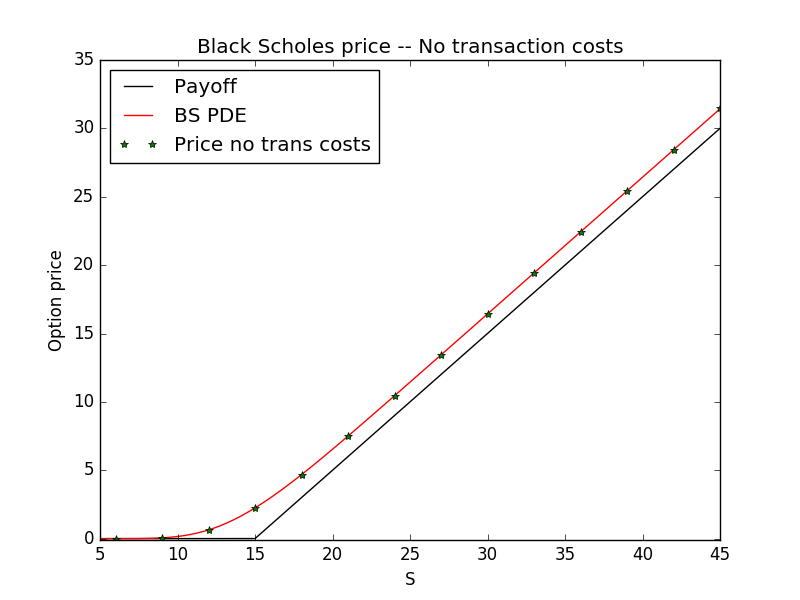
\includegraphics[width=\linewidth]{BS_No_costs.png}
   \caption{Writer prices with zero transaction costs for diffusion process. Parameters are in the table \ref{tab:BS}.}
   \label{Fig1} 
 \end{minipage}
 \ \hspace{2mm} \hspace{3mm} \
 \begin{minipage}[b]{0.5\linewidth}
  \centering
   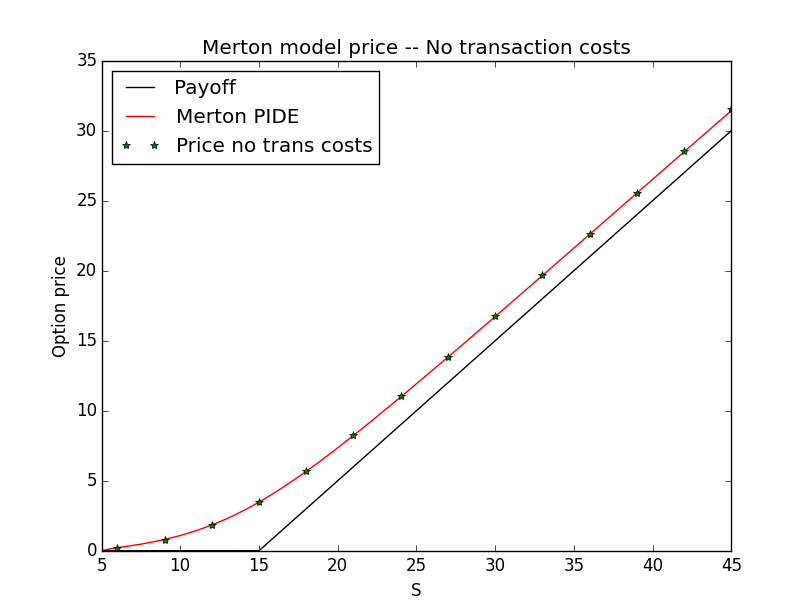
\includegraphics[width=\linewidth]{no_costs.png}
   \caption{Writer prices with zero transaction costs for Merton process. Parameters are in the table \ref{tab:Mert}.}
   \label{Fig2}
 \end{minipage}
  \ \hspace{2mm} \hspace{3mm} \
  \begin{minipage}[b]{\linewidth}
  \centering
   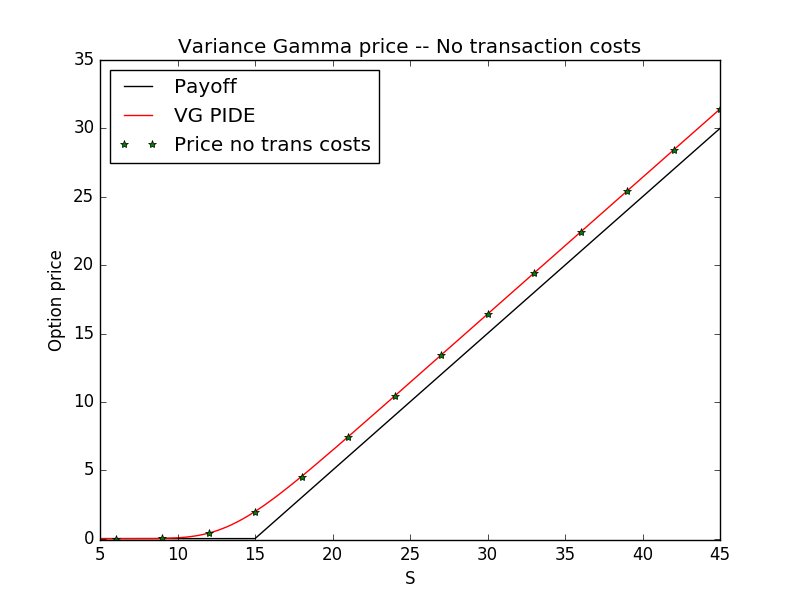
\includegraphics[width=0.55\linewidth]{No_costs_VG.png}
   \caption{Writer prices with zero transaction costs for VG process. Parameters are in the table \ref{tab:VG}.}
   \label{Fig3}
 \end{minipage}
\end{figure}
The processes parameters and the option details are collected in the tables \ref{tab:BS}, \ref{tab:Mert} and \ref{tab:VG}.
We compute the option prices using the standard 
\emph{martingale pricing theory} (see chapter \ref{Chapter2}). In the table \ref{tab:ATM_price} we show the \emph{at the money} values obtained with the closed formula 
and by solving the respective PIDE. 
The closed formula for the diffusion process is the well known \cite{BS73} formula. To compute the Merton price we use the series approximation formula derived in \cite{Me76},
and for the VG price we used the semi-closed formula derived in \cite{MCC98}. The PIDE prices are obtained by solving the Eqs. (\ref{BS_PDE}), (\ref{Merton_PIDE}) and (\ref{VG_PIDE}).
Of course, the parameter $\mu$ has not been used to compute the prices in Tab. \ref{tab:ATM_price}. We will prove with a numerical test that
even though the portfolio process (\ref{portfolio_dynamics2}) has a drift parameter $\mu$, it does not play an important role for the option price.
\begin{table}[h!]
\begin{center}
\begin{minipage}{0.8\linewidth}
\centering
 \begin{tabular}{||l|l|l||l|{c}||r||}
 \hline
  \multicolumn{6}{|c|}{Diffusion parameters} \\
  \hline
  $K$ & $T$ & $r$ & $\mu$ & $\sigma$ & $\gamma$ \\
  \hline
  15 & 1 & 0.1 & 0.1 & 0.25 & 0.001 \\
  \hline
  \end{tabular}
  \caption{This table shows option's parameters and diffusion process parameters.}
  \label{tab:BS}
\end{minipage}
 \end{center}
\end{table}
\begin{table}[h!]
 \begin{center}
 \begin{minipage}{0.8\linewidth}
  \centering
  \begin{tabular}{||l|l|l||l|l|l|l|{c}||r||}
  \hline
  \multicolumn{9}{|c|}{Merton parameters} \\
  \hline
  $K$ & $T$ & $r$ & $\mu$ & $\sigma$ & $\alpha$ &$\xi$ & $\lambda$ & $\gamma$\\
  \hline
  15 & 1 & 0.1 & 0.1 & 0.25 & 0 & 0.5 & 0.8 & 0.04\\
  \hline
  \end{tabular}
  \caption{This table shows option's parameters and Merton process parameters.}
  \label{tab:Mert}
 \end{minipage}
 \end{center}
\end{table}
\begin{table}[h!]
\begin{center}
 \begin{minipage}{0.8\linewidth}
  \centering
 \begin{tabular}{||l|l|l|l||l|l|{c}||r||}
\hline
  \multicolumn{8}{|c|}{VG parameters} \\
 \hline
$K$ & $T$ & $r$ & $\mu$ & $\theta$ & $\sigma$ &$\kappa$ & $\gamma$ \\
\hline
15 & 1 & 0.1 & 0.1 & -0.1 & 0.2 & 0.1 & 0.05 \\
\hline
\end{tabular}
  \caption{This table shows option's parameters and VG process parameters.}
  \label{tab:VG}
\end{minipage}
  \end{center}
\end{table}

In the following analysis, we consider the PIDE prices as our benchmarks for comparisons.   
In all the computations we use equal transaction costs for buying and selling, $\theta_b = \theta_s$.

In Fig. \ref{Fig1}, \ref{Fig2} and \ref{Fig3} we show that model prices replicate the PIDE prices for zero transaction costs and small values of $\gamma$. 
The values of $\gamma$ in the tables \ref{tab:BS},
\ref{tab:Mert}, \ref{tab:VG} are chosen very small\footnote{ In chapter 5 of \cite{GK99} are presented some common values for the risk aversion coefficient: $\gamma=0.3$, $\gamma=0.2$ and $\gamma=0.1$ for high, medium and low level of risk aversion respectively.}. 
An intuitive argument to justify this choice is that for $\gamma \to 0$, the utility function 
can be approximated by a linear utility $\mathcal{U}(w) = 1 - e^{-\gamma w} \approx \gamma w$ and the investor is considered risk neutral. 
For more details we refer to \cite{Carmona} and references therein. 
\begin{figure}[t!]
 \begin{minipage}[b]{0.5\linewidth}
   \centering
   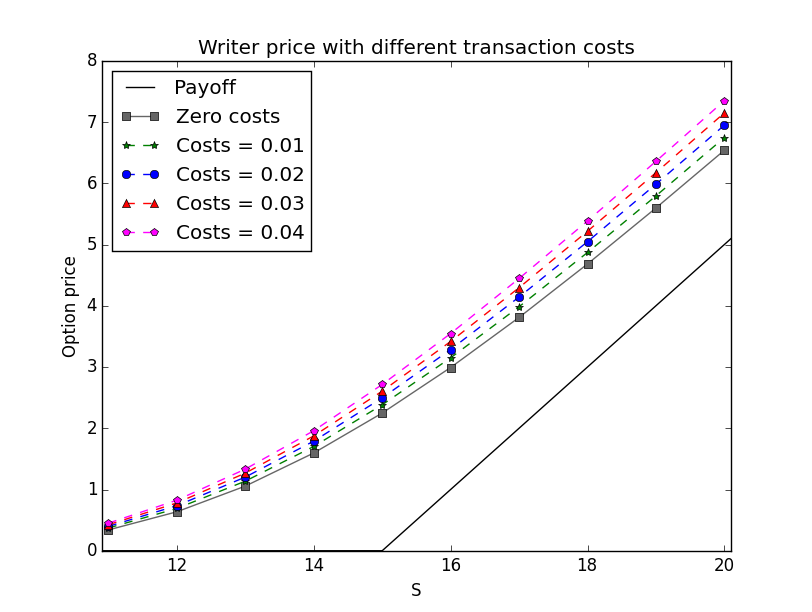
\includegraphics[width=\linewidth]{Trinomial_writer.png}
   \caption{Writer prices for different transaction costs. The continuous line is the solution of the Black-Scholes PDE.}
   \label{Fig4} 
 \end{minipage}
 \ \hspace{2mm} \hspace{3mm} \
 \begin{minipage}[b]{0.5\linewidth}
  \centering
   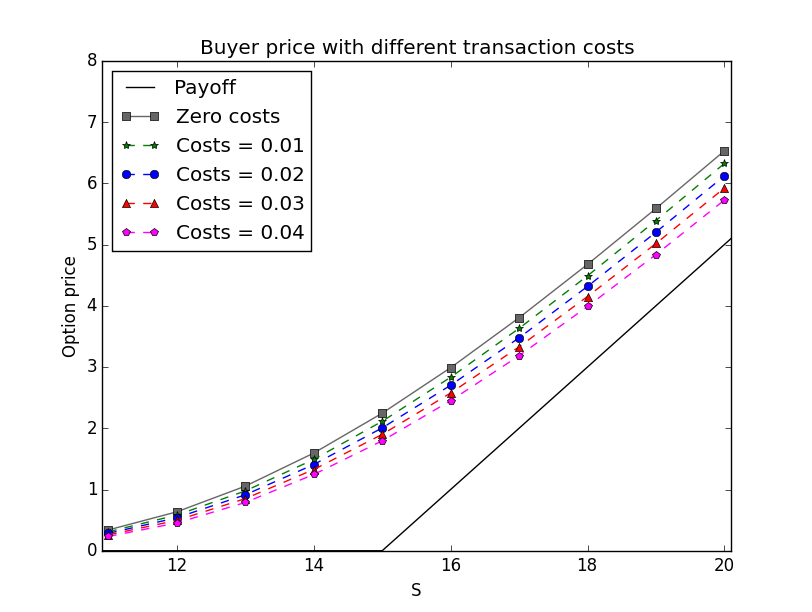
\includegraphics[width=\linewidth]{Trinomial_buyer.png}
   \caption{Buyer prices for different transaction costs. The continuous line is the solution of the Black-Scholes PDE.}
   \label{Fig5}
 \end{minipage}
\end{figure}
\begin{table}[h!]
\begin{center}
\begin{minipage}{\linewidth}
\centering
 \begin{tabular}{||l|r|r|r||}
 \hline
  \multicolumn{4}{|c|}{Convergence table} \\
  \hline
  $N = \bar M$ & Price with $\gamma = 0.0001$ & Price with $\gamma = 0.001$ & Price with $\gamma = 0.01$\\
  \hline
    50 & 2.2412146517 & 2.2417649462 & 2.2473119666 \\
  \hline
    100 & 2.2491427418 & 2.2495065494 & 2.2531593006 \\
  \hline  
    200 & 2.2454227575 & 2.2456761615 & 2.2482167262 \\
  \hline
    400 & 2.2467842126 & 2.2469596683 & 2.2487172682 \\
  \hline
    800 & 2.2461889356 & 2.2462711875 & 2.2476351737 \\
  \hline
    1600 & 2.2465769781 & 2.2466622275 & 2.2475154717 \\
  \hline
    3200 & 2.2464120247 & 2.2464716771 & 2.2470685805 \\
  \hline
    3500 & 2.2463661466 & 2.2464231225 & 2.2469932278 \\
  \hline
  \end{tabular}
  \caption{Convergence table for ATM diffusion prices ($\bar L = 3$) with zero transaction costs.}
  \label{tab:convergence}
\end{minipage}
 \end{center}
\end{table}

\subsection{Diffusion results}

In the figures \ref{Fig4} and \ref{Fig5} we show the writer and buyer prices with different values
of transaction costs, for the diffusion process with parameters in Tab. \ref{tab:BS}.  
We can see that a higher transaction cost corresponds to a higher writer price, while a lower transaction cost corresponds to a lower buyer price.
Indeed, the writer and buyer prices are respectively increasing and decreasing functions of the transaction cost, as already verified in \cite{ClHo97}.

The values obtained in figures \ref{Fig1},\ref{Fig4},\ref{Fig5} are calculated with $N=1500$ time steps and $\bar M = N$. 
In the Table \ref{tab:convergence} we show the ATM option prices with $\theta_s = \theta_b = 0$, and different values of risk aversion $\gamma = 0.0001$, 
$\gamma = 0.001$ and $\gamma = 0.01$.
The prices are very close to the Black-Scholes price in table \ref{tab:ATM_price}, 
and even using values of gamma that have one or two orders of magnitude of difference, the option prices only change at the fourth decimal digit. 
Since we do not know the limit price for $N \to \infty$, we can assume it is the price computed for $N=3500$, and through the values in Table \ref{tab:convergence} 
estimate the rate of convergence. 

\subsection{Merton results}

\begin{figure}[t!]
 \begin{minipage}[b]{0.5\linewidth}
   \centering
   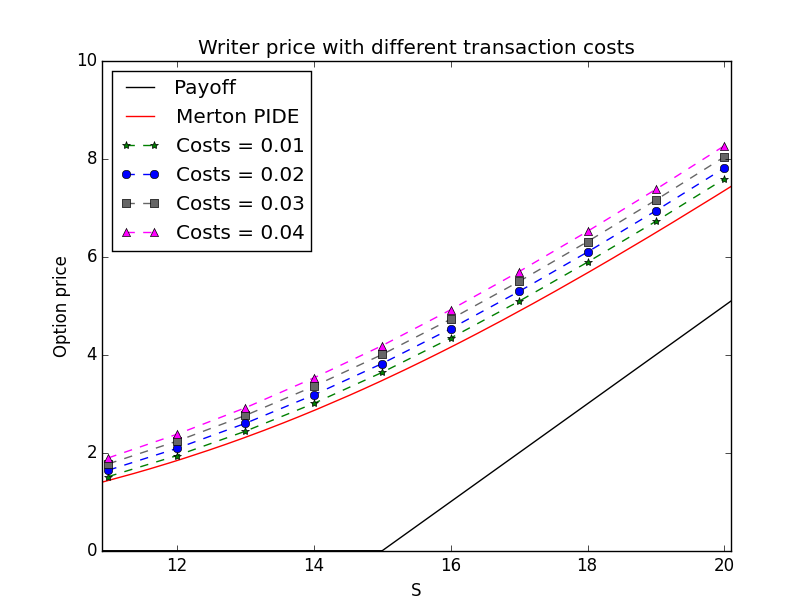
\includegraphics[width=\linewidth]{writer_cost.png}
   \caption{Writer prices for different transaction costs. The continuous line is the solution of the Merton PIDE.}
   \label{Fig6} 
 \end{minipage}
 \ \hspace{2mm} \hspace{3mm} \
 \begin{minipage}[b]{0.5\linewidth}
  \centering
   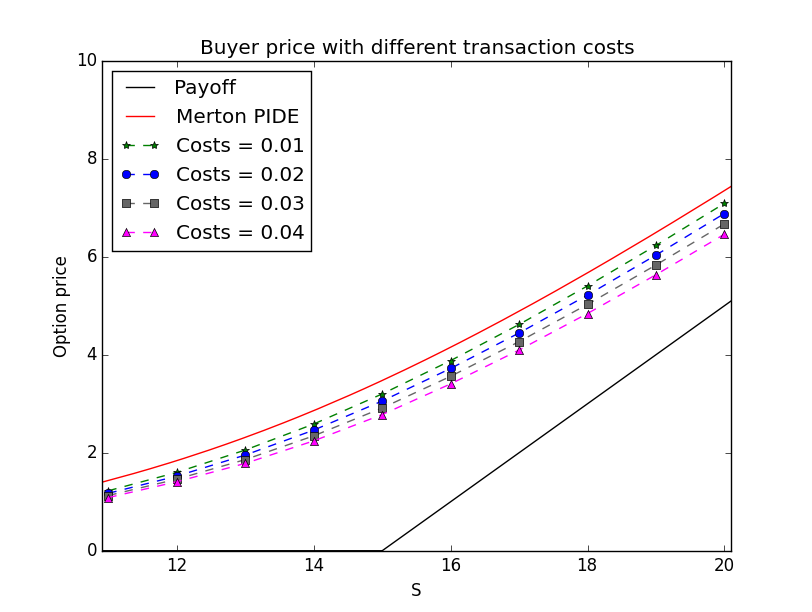
\includegraphics[width=\linewidth]{Price_buyer.png}
   \caption{Buyer prices for different transaction costs. The continuous line is the solution of the Merton PIDE.}
   \label{Fig7}
 \end{minipage}
\end{figure}
In the Figures \ref{Fig6} and \ref{Fig7} we show the writer and buyer prices for the Merton process, with parameters in Tab. \ref{tab:Mert}.
An interesting feature of the multinomial tree construction for jump-diffusion processes is that $\bar L \propto \sqrt{N}$.
The integral domain is restricted to the bounded domain $[-B_1,B_2]$ with length $B_1+B_2 = \bar L \, h_x$. 
The size of a space step is $h_x = \sqrt{\E[\Delta X^2]} = \sqrt{( \sigma^2 + \lambda \xi^2 + \lambda \alpha^2 ) \, \Delta t}
= \sigma_X \sqrt{\Delta t}$ (see Eq. (\ref{loc1})).
However, the size of the Poisson jumps does not scale with $\Delta t$. So the number $\bar L$ has to be chosen big enough in order 
to have $L\, h_x \geq B_1+B_2$. 
For a fixed $h_x$, the interval $[-B_1,B_2]$ should be as big as possible, but the choice of the truncation depends on the shape of the L\'evy measure.  
The figures \ref{Fig13}, \ref{Fig14} show two examples where we choose $[-B_1,B_2] = [\xi,\xi]$ and $[-B_1,B_2] = [-3\xi,3\xi]$ respectively. These choices correspond to 
$\bar L = 19$ and $\bar L = 59$.
For the Merton L\'evy measure (a scaled Normal distribution), a good choice is $[-B_1,B_2] = [-3\xi,3\xi]$, with length $\bar L \, h_x = 6\xi$. 
It is well known that the integral over this region is about the $99.74\%$ of the total area.      
Using this interval and the parameters in Tab. \ref{tab:Mert} we obtain the relation $\bar L \geq 5.86 \sqrt{N}$ that relates $N$ and $\bar L$.
In the calculation of the Merton prices in Figures \ref{Fig6} and \ref{Fig7}, we used a discretization with $N=\bar M =100$, and $\bar L = 81$, 
with a good balance between small computational time and small price error. 
\begin{table}[h!]
\begin{center}
\begin{minipage}{\linewidth}
\centering
 \begin{tabular}{||l||c|c|c|c|c||}
 \hline
  \multicolumn{6}{|c|}{Truncation error table} \\
  \hline
  $N$ & $\bar L=51$ &   $\bar L=71$   & $\bar L=91$ & $\bar L=101$ & $\bar L=111$ \\
  \hline
    50 &  3.4813187161  & 3.4816163394  & 3.4816170496  & 3.4816170504 & 3.4816170504  \\
  \hline
    100  & 3.4687744548 & 3.4788060527 &  3.4791415876  & 3.4791464725 & 3.4791469712  \\
  \hline  
    150  & 3.4390903586 & 3.4744039174 & 3.4775744098 & 3.4777147784 & 3.4777420291  \\
  \hline  
    200  & 3.3994424401 & 3.4663389997 & 3.4764398666 & 3.4772345512 & 3.4774570321 \\
  \hline
  \end{tabular}
  \caption{Truncation error table for ATM Merton prices with zero transaction costs. Parameters in Tab. \ref{tab:Mert}. For increasing $\bar L$, 
  the truncation error in the prices decreases.}
  \label{tab:convergence2}
\end{minipage}
 \end{center}
\end{table}\\
In Tab. \ref{tab:convergence2} we show different Merton prices for zero transaction costs and different values of $N$ and $\bar L$.
Looking at the table from left to right, for each fixed $N$ it is possible to note how the truncation error decreases when $\bar L$ increases.
\begin{table}[h!]
\begin{center}
\begin{minipage}{0.8\linewidth}
\centering
 \begin{tabular}{||c|c|c||}
 \hline
  \multicolumn{3}{|c|}{Convergence table} \\
  \hline
  $N = \bar M$ & $\bar L$ & Price \\
  \hline
    50 & 61 & 3.4816000776 \\
  \hline
    75 & 75 & 3.4799801710  \\
  \hline  
    100 & 91 & 3.4791415876  \\
  \hline
    125 & 97 & 3.4782540801 \\
  \hline   
    150 & 105 & 3.4777312502  \\
  \hline
    175 & 113 & 3.4776103369 \\ 
  \hline
    200 & 121 & 3.4775134685  \\
  \hline
  \end{tabular}
  \caption{Convergence table for ATM Merton prices with zero transaction costs.}
  \label{tab:convergence3}
\end{minipage}
 \end{center}
\end{table}\\
In Table \ref{tab:convergence3} we show several prices with increasing values of $N$ and $\bar L$. We choose $\bar L$ big enough, such that the truncation error can be ignored.
In a convergence analysis, the price with $N=200$, $\bar L = 121$ can be considered as the limit value. Given the high computational complexity of the algorithm, 
it is difficult to present prices with bigger values of $N$,$\bar L$.
For larger values of $N$ and smaller $\gamma$, we expect a convergence to the Merton price in Tab. \ref{tab:Mert}. 

\subsection{VG results}\label{num_sec_VG}

\begin{figure}[t!]
 \begin{minipage}[b]{0.5\linewidth}
   \centering
   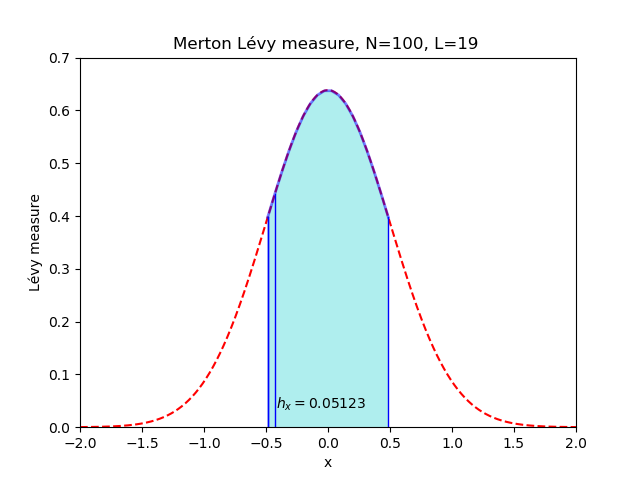
\includegraphics[width=\linewidth]{Mert61_3.png}
   \caption{Merton L\'evy measure computed using parameters in Tab. \ref{tab:Mert}, $N=100$ and $\bar L=19$. 
   The domain $[-B_1,B_2] = [-\xi,\xi]$ has length $\bar L h_x \approx 2 \xi$.}
   \label{Fig13} 
 \end{minipage}
 \ \hspace{2mm} \hspace{3mm} \
 \begin{minipage}[b]{0.5\linewidth}
  \centering
   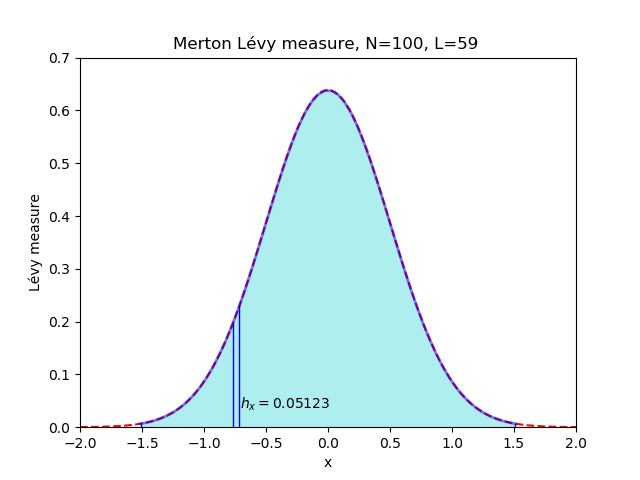
\includegraphics[width=\linewidth]{Mert101_3.png}
   \caption{Merton L\'evy measure computed using parameters in Tab. \ref{tab:Mert}, $N=100$ and $\bar L=59$. 
   The domain $[-B_1,B_2] = [-3\xi,3\xi]$ has length $\bar L h_x \approx 6 \xi$.}
   \label{Fig14}
 \end{minipage}
\end{figure}
\begin{figure}[t!]
 \begin{minipage}[b]{0.5\linewidth}
   \centering
   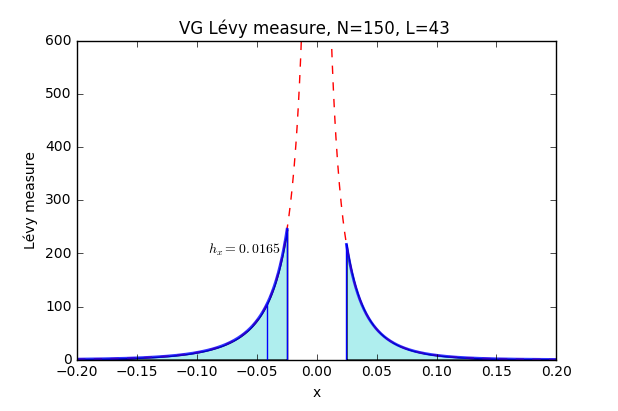
\includegraphics[width=\linewidth]{VG43.png}
   \caption{VG L\'evy measure computed using parameters in Tab. \ref{tab:VG}, $N=150$ and $\bar L=43$. 
   The domain $[-B_1,-\epsilon]\bigcup [\epsilon,B_2]$ has length $(\bar L-3) h_x$. The highlighted area is $99.9\%$ of the total area.}
   \label{Fig15} 
 \end{minipage}
 \ \hspace{2mm} \hspace{3mm} \
 \begin{minipage}[b]{0.5\linewidth}
  \centering
   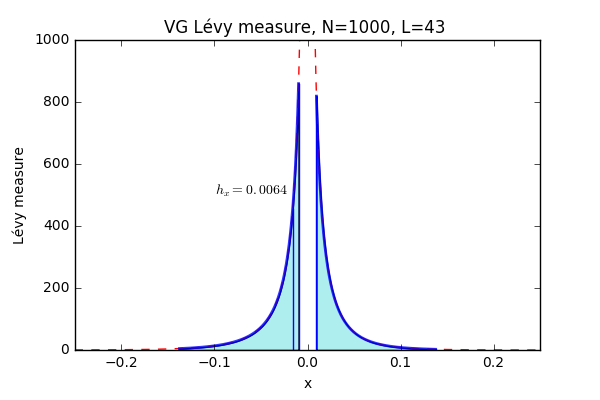
\includegraphics[width=\linewidth]{VG1000.png}
   \caption{VG L\'evy measure computed using parameters in Tab. \ref{tab:VG}, $N=1000$ and $\bar L=43$. 
   The domain $[-B_1,-\epsilon]\bigcup [\epsilon,B_2]$ has length $(\bar L-3) h_x$. The highlighted area is $98.9\%$ of the total area.}
   \label{Fig16}
 \end{minipage}
\end{figure}

In the Figures \ref{Fig8} and \ref{Fig9} we show how the writer and buyer prices for the VG process change for several level of transaction costs (parameters in Tab. \ref{tab:VG}). 
In the computations we used $N=\bar M = 150$ and $\bar L = 43$. Under this choice the program runs in a reasonable computational time. 
The integration region in \ref{VG_gen} is restricted to $[-B_1,-\epsilon]\bigcup [\epsilon,B_2]$ with $\epsilon=1.5h_x$. The choice of $B_1$ and $B_2$ depends on the shape of the 
L\'evy measure. 
In Fig. \ref{Fig15} and \ref{Fig16} we show two examples for the VG L\'evy measure (using parameters in table \ref{tab:VG}) with $N=150$, $h_x=0.0165$ and $N=1000$, $h_x=0.0064$. 
The two L\'evy measures are normalized, such that the integral on the region $[-\infty,-\epsilon]\bigcup [\epsilon,+\infty]$ equals one, and the 
area underlying the functions on $[-B_1,-\epsilon]\bigcup [\epsilon,B_2]$ is highlighted.
We can see that in both cases, using $\bar L = 43$, it is possible to cover a very high percentage of the initial unrestricted region. We can conclude that, unlike the Merton
measure, we do not need a big truncation interval.
Given the space step $h_X = \sigma_X\sqrt{\Delta t}$, with  
$ \sigma_X = \sqrt{\sigma_J^2 + \sigma_{\epsilon}^2} = \sqrt{\sigma^2+\theta^2 \kappa}$ 
and $\Delta t = T/N$, it is enough to require a region at least as big as the standard deviation of the jump process: 
$h_X \bar L > \sigma_J$, where  
$\sigma_J^2 = \int_{|z| \geq \epsilon} z^2 \nu(dz) $.
Putting all together, the relation becomes $\bar L\geq \frac{\sigma_J}{\sigma_X} \sqrt{N}$, and replacing the values $\sigma_X = 0.2024$ and $\sigma_J=0.1916$ 
we get $\bar L \geq 0.94 \sqrt{N}$.
\begin{table}[h!]
\begin{center}
\begin{minipage}{0.8\linewidth}
\centering
 \begin{tabular}{||c|c|c||}
 \hline
  \multicolumn{3}{|c|}{Convergence table} \\
  \hline
  $N = \bar M$ & $\lambda_{\epsilon}$ & Price \\
  \hline
    50 & 4.73 & 1.9109347161 \\
  \hline
    100 & 7.82 & 1.9578065378  \\
  \hline  
    150 & 10.01 & 1.9820789189  \\
  \hline
    200 & 11.73 & 1.9961807305 \\
  \hline   
    250 & 13.14 & 2.0047194603  \\
  \hline
    300 & 14.35 & 2.0085360317 \\ 
  \hline
    350 & 15.40 & 2.0094361889  \\
  \hline
  \end{tabular}
  \caption{Convergence table for ATM VG prices with $\bar L =43$, zero transaction costs and parameters in Tab \ref{tab:VG}.}
  \label{tab:convergence4}
\end{minipage}
 \end{center}
\end{table}\\
In the Table \ref{tab:convergence4} we present several option prices computed with different values of $N$, but with fixed $\bar L$.
In the case of the VG process it is more difficult to analyze the convergence results.
This is due to the approximation (\ref{log_sde_inf_act2}) introduced to replace the infinite activity jump component with a Brownian motion. All the new parameters
(\ref{sig_eps}) depend on $\epsilon$, and consequently on $N$.
Within our discretization ($N=150$), we have $\sigma_{\epsilon} = 0.0654$, $\lambda_{\epsilon} = 10.01$. 
With those parameters we obtain an ATM price for zero transaction costs of 1.9821, which is very close the the PIDE price in Tab. \ref{tab:ATM_price}. 
We expect to have convergence to the PIDE price for $N\to \infty$ and $\gamma\to0$.\\
When $N \to \infty$ and $\epsilon \to 0$, the parameters $\sigma_{\epsilon} \to 0$ and $\lambda_{\epsilon}\to \infty$.
For each $N$ it is important to verify that the stability conditions $(1-\lambda_{\epsilon} \Delta t)>0$ and $h_x^2 > \sigma_{\epsilon}^2 \Delta t$ are always satisfied, 
in order to have a consistent Markov chain approximation.
The main problems are the high dependence of the price on the parameter $\epsilon$ and therefore on the discretization step $h_x$, together with the high complexity of the algorithm.
For instance, with $N=\bar M=1000$ and $\bar L = 43$ the program takes more than two hours to run. 
The convergence of the approximated process (\ref{log_sde_inf_act2}) to the original VG process is very slow, and this is reflected in the convergence 
of the VG PIDE (\ref{VG_PIDE}).
In order to solve it (using the IMEX scheme proposed by \cite{CoVo05b}) we constructed
a grid with 13000 space steps of size $\delta x = 0.0004$ and 7000 time steps, and obtained the price in Tab \ref{tab:ATM_price}, 
with the approximated activity $\lambda_{\epsilon} = 75$.
Consequently, we expect to have good convergence results in our algorithm when $N\sim 10^4$.
All the presented prices (Figures \ref{Fig8} and \ref{Fig9}) have thus a truncation error, which is ``hidden'' by an accurate choice of the value $\gamma$. 
We refer to \cite{CoVo05b} for a detailed error analysis.
\begin{figure}[t!]
 \begin{minipage}[b]{0.5\linewidth}
   \centering
   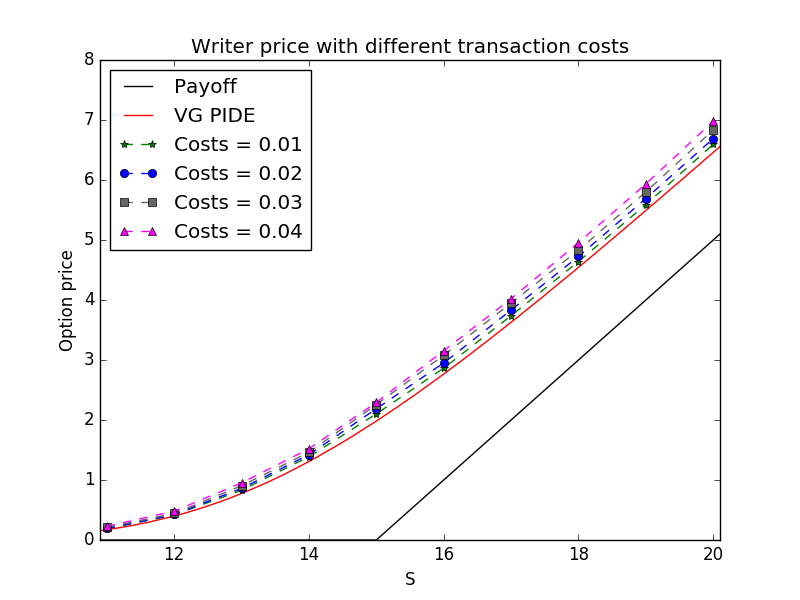
\includegraphics[width=\linewidth]{VG_Writer.png}
   \caption{Writer prices for different transaction costs. The continuous line is the solution of the VG PIDE.}
   \label{Fig8} 
 \end{minipage}
 \ \hspace{2mm} \hspace{3mm} \
 \begin{minipage}[b]{0.5\linewidth}
  %\centering
   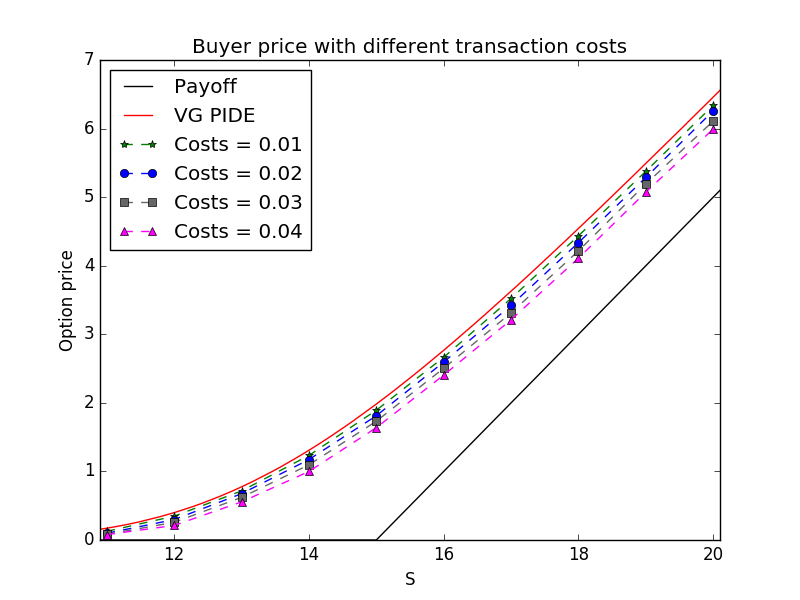
\includegraphics[width=\linewidth]{VG_Buyer.png}
   \caption{Buyer prices for different transaction costs. The continuous line is the solution of the VG PIDE.}
   \label{Fig9}
 \end{minipage}
\end{figure}  

\subsection{Properties of the model}\label{model_properties}

In this section we want to analyze the properties of the model and how the option price depends on the level of transaction costs $\theta_b$, $\theta_s$, 
the risk aversion parameter $\gamma$ and the drift $\mu$. 
We use the Merton process with parameters of Tab. \ref{tab:Mert} to test the properties.
In Tab. \ref{tab:costs} we show the writer ATM option values for different transaction costs in Fig. \ref{Fig3}.  
\begin{table}[h!]
\begin{center}
 \begin{minipage}{\linewidth}
  \centering
 \begin{tabular}{||l||c|c|c|c|c||}
\hline
 & cost = 0 & cost = 0.01 & cost = 0.02 & cost = 0.03 & cost = 0.04  \\
\hline
Merton & 3.4771 & 3.6400 & 3.8212 & 4.0054 & 4.1864 \\
\hline
VG & 1.9821 & 2.0921 & 2.1870 & 2.2568 & 2.3131 \\
\hline
\end{tabular}
  \caption{Merton and VG writer prices for different transaction costs, with parameters as in Tab. (\ref{tab:Mert}), (\ref{tab:VG}). }
  \label{tab:costs}
\end{minipage}
  \end{center}
\end{table}
In Fig. \ref{Fig10} we can see better how the price for the writer is affected by the change of the transaction costs. 
The picture shows prices for different values of risk coefficient.
The risk profile of the investor also plays an important role. As already shown in \cite{HoNe89}, the writer option price is an
increasing function of the risk aversion. 
The Figure \ref{Fig11} confirms their results.

In all the previous computations we always used the drift term $\mu$ equal to the risk free interest rate $r$. This is the same choice  
of \cite{HoNe89}. They do not explain the reasons for their choice, but follow the common practice used in the standard no-arbitrage
theory, based on the fact that
the option price has to be independent of the expected return of the underlying asset.
It turns out that this fact is still true in this model, as we can see in Fig. \ref{Fig12}. This feature
of the model has been analyzed in \cite{Damgaard} for the diffusion case. This numerical experiment confirms that the option prices 
are not very sensitive to the change of the drift $\mu$.

\begin{figure}[t!]
 \begin{minipage}[b]{0.5\linewidth}
   \centering
   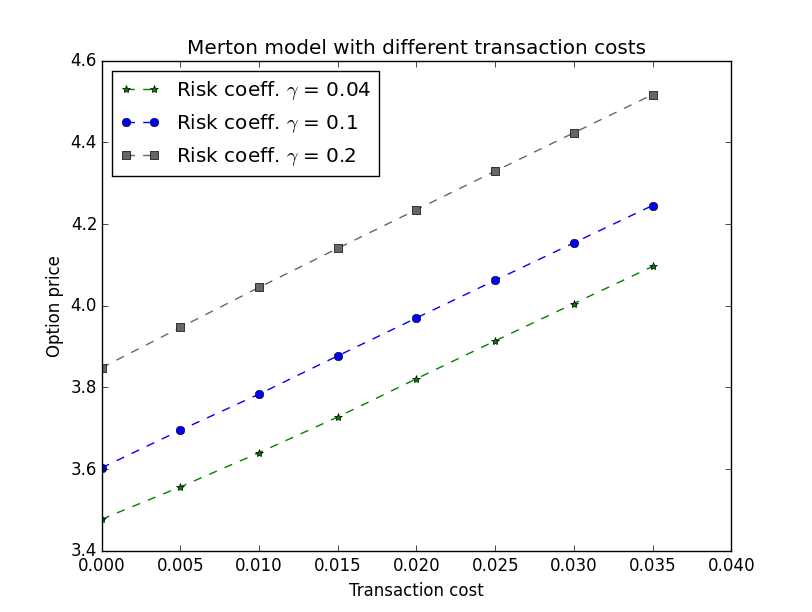
\includegraphics[width=\linewidth]{P_vs_cost.png}
   \caption{Merton option prices for the writer as function of the transaction cost, with different values of $\gamma$.}
   \label{Fig10} 
 \end{minipage}
 \ \hspace{2mm} \hspace{3mm} \
 \begin{minipage}[b]{0.5\linewidth}
  \centering
   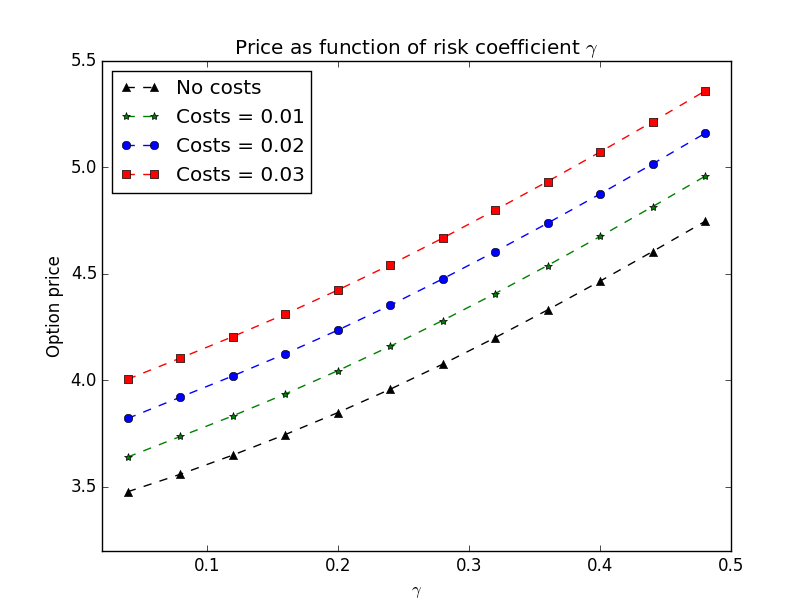
\includegraphics[width=\linewidth]{price_gamma.png}
   \caption{Merton option prices for the writer as function of $\gamma$, with different values of transaction costs.}
   \label{Fig11}
 \end{minipage}
  \ \hspace{2mm} \hspace{3mm} \
  \begin{minipage}[b]{\linewidth}
  \centering
   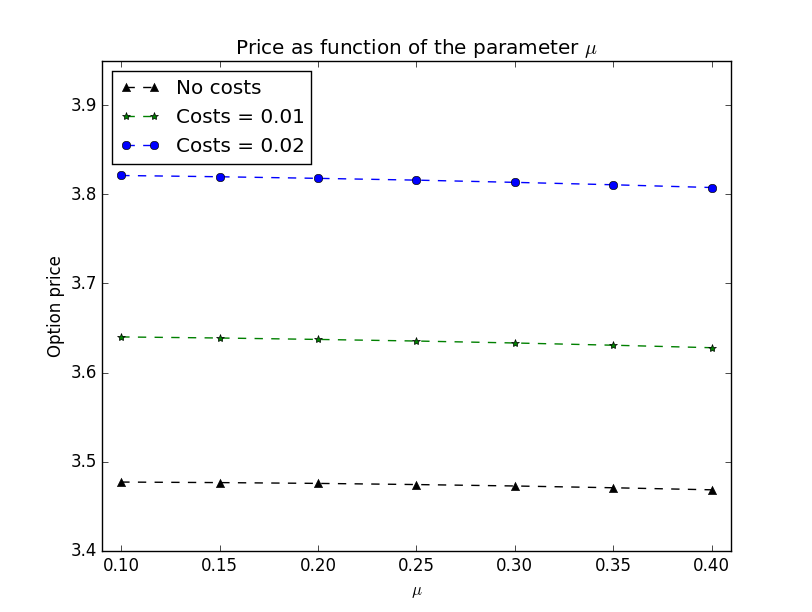
\includegraphics[width=0.55\linewidth]{price_mu2.png}
   \caption{Merton option prices for the writer as function of $\mu$, with different values of transaction costs.}
   \label{Fig12}
 \end{minipage}
\end{figure}



\section{Solution of the problem with no variable reduction}


Another approach to the problem is to solve the original HJB equation \ref{HJB1}. 
A few authors have already presented some results for the diffusion case, i.e. \cite{Song14} and \cite{Pal15}, but the performances are poor and the results are not very satisfactory.

However, if we want to include the default feature, we have to deal with the four-dimensional original problem. In the variable reduction section \ref{reduction_sec}
we assumed such a high value of credit availability $C$, such that the default probability can be ignored. 
In the following we work with the original problem and derive a discrete time dynamic programming equation as done when we obtained (\ref{HJB3}).\\
The discretized SDE for the cash account process $B_t$ (\ref{BT}) is:
\begin{equation}
 B_{n+1} =  e^{r \Delta t} \biggl( B_n - (1+\theta_b) e^{X_n} \Delta L_n + (1-\theta_s) e^{X_n} \Delta M_n \biggr)
\end{equation}

Let us derive the backward algorithm for computing the value function using the dynamic programming equation. The integral representation of \ref{HJB1} is:
\begin{align}\label{HJB4}
 V(t,b,y,x) = \max & \; \biggl\{ \E_{b,y,x} 
 \biggl[ V \bigl( t+\Delta t, b e^{r \Delta t}, y, x + \Delta X \bigr) \biggr], \\ \nonumber
 & \max_{\Delta L_t} \biggl[ V \bigl( t,b-e^x(1+\sigma_b)\Delta L_t , y+\Delta L_t, x \bigr) \biggr] , \\ \nonumber
 & \max_{\Delta M_t} \biggl[ V \bigl( t,b+e^x(1-\sigma_s)\Delta M_t , y-\Delta M_t, x \bigr) \biggr]
 \biggr\}.
\end{align}
Using the same argument that led (\ref{HJB25}) to (\ref{HJB3}),
we can represent the value function at time $t$, as an expectation of its values at time $t+\Delta t$. 
We obtain the discrete DPE: 
\begin{align}\label{HJB5}
 & V(t_n,B_n,Y_n,X_n) = \max \; \biggl\{ \E_n 
 \biggl[ V \bigl( t_{n+1}, e^{r \Delta t} B_n, Y_n, X_n + \Delta X_n \bigr) \biggr], \\ \nonumber
 & \max_{\Delta L_n} 
 \E_n \biggl[ V \bigl( t_{n+1}, e^{r\Delta t}(B_n - e^{X_n}(1+\sigma_b)\Delta L_n) , Y_n + \Delta L_n, X_n + \Delta X_n \bigr) \biggr] , \\ \nonumber
 & \max_{\Delta M_n}
 \E_n \biggl[ V \bigl( t_{n+1}, e^{r\Delta t}(B_n + e^{X_n}(1-\sigma_s)\Delta M_n) , Y_n - \Delta M_n, X_n + \Delta X_n \bigr) \biggr]
 \biggr\},
\end{align}
where all the expectations are conditioned on the current state $(B_n,Y_n,X_n)$. \\

\begin{figure}[t!]
   \centering
   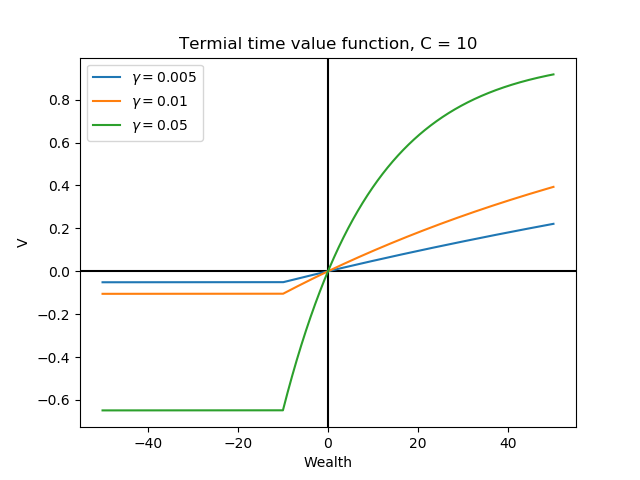
\includegraphics[width=0.7\linewidth]{terminal_utility.png}
   \caption{Terminal time value functions.}
   \label{Fig21} 
\end{figure}
The algorithm is almost the same of that explained in Section \ref{algorithm_Sect}. Here we highlight the differences (see \cite{Pal15}):
\begin{enumerate}
 \item Create the lattice for the log-price $X_n$ with step sizes $h_x$, where each node has $\bar L = \#(\Sigma_x) = K_1 + K_2 +1$ branches.
 \item Create the shares vector $Y$ with discretization step $h_y$. Its dimension is $\bar M = \#(\Sigma_y) = K_3+K_4+1$.
 \item Create the cash vector $B$ with discretization step $h_b$. Its dimension can be chosen equal to $\bar M$ for simplicity.
 \item Evaluate the value functions at terminal time. It is a three-dimensional grid with dimension $\bigl( N(\bar L-1)+1 \bigl) \times \bar M \times \bar M$.
 \item Create a backward loop over time, with index $n$ that starts at $N$ and finishes at $1$.
 \item Create a loop over all $x \in X_n$, $y \in Y$ and $b \in B$.
 \item Given the function $V(n+1)$, find the highest value in (\ref{HJB5}) obtained over all values $\Delta L, \Delta M$ such that:
 $$y + \Delta L \in Y \quad \mbox{and} \quad y - \Delta M \in Y, $$ 
 $$ e^{r\Delta t} (b - e^{x}(1+\sigma_b)\Delta L) \geq e^{r\Delta t} \min(B)$$ 
 $$ e^{r\Delta t} (b + e^{x}(1-\sigma_s)\Delta M) \leq e^{r\Delta t} \max(B) $$
 The values of $V$ need to be obtained by interpolation.
 \item Solve numerically the formulas (\ref{writer_p}) or (\ref{buyer_p}) to find the option price.      
\end{enumerate}
The algorithm is very expensive. Since it has one degree of freedom more than the algorithm in Section \ref{algorithm_Sect}, the computational complexity is 
$\mathcal{O}\biggl( (N+1)\bigl[\frac{N(\bar L-1)}{2}+1 \bigr] \times \bar M \times \bar M \times \bar M \biggr)$.

In figure (\ref{Fig21}) it is possible to see how the terminal time value function (see (\ref{max_probl1})) behaves for different values of gamma.
The main difference between (\ref{max_probl1}) and (\ref{DPZ_max_probl0}) is that the value function is no more concave. 
Moreover in the points $(b,y,x)$ such that $\mathcal{W} = -C$, the function is not differentiable, and this may create instabilities in the numerical computations.

In the following we compute the value function for a Merton process with values in table \ref{tab:Mert}. 
We choose $-20 \leq B \leq 20$, and consider values of $N = \bar M = 25$ and $\bar L = 11$. 
Even with these small values, the algorithm takes about 4 hours to run. 
I wrote the algorithm in Python (using numpy arrays) and I ran the program on a Linux machine with a i7 processor. I think that in order to increase the speed of the program
it is necessary to write the program in a low level language such as C of Fortran.
\begin{figure}[t!]
   \centering
   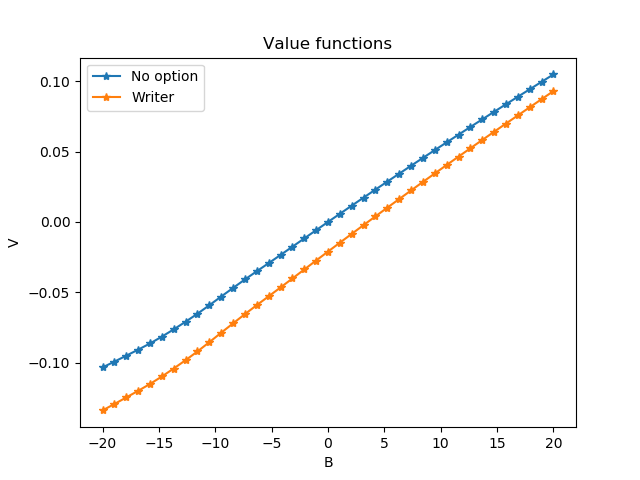
\includegraphics[width=0.6\linewidth]{value_f_C5000.png}
   \caption{Value function for the writer and value function with no option at time $t_0$ with $Y_0=0$ and $S_0=15$. The option price at $B=0$ is $p^w=3.48303858$.}
   \label{Fig22} 
\end{figure}

In the figure \ref{Fig22} we computed the value functions and the option prices for a very high value of $C$. We chose $C= 5000$.
The value functions are quite smooth and, as expected, the option price (obtained by inverting the formula (\ref{writer_p}) ) is not affected too much by the initial wealth. 
The high value of the credit availability $C$ 
has to be intended as a low default probability. Therefore the problem leads back to the problem with 3 variables. And the numerical results confirm it.

A different story happens when we choose a small credit availability. For example $C = 10$.\\ 
In figure \ref{Fig23} we can see that the two value functions have the same value for $B<-C$, because in this region the value function corresponds to the boundary conditions
(remember that we are considering $Y_0=0$). 
For higher values of $B$,the influence of the boundary conditions decreases and the value functions look like those in figure \ref{Fig22}.
\begin{figure}[t!]
 \begin{minipage}[b]{0.5\linewidth}
   \centering
   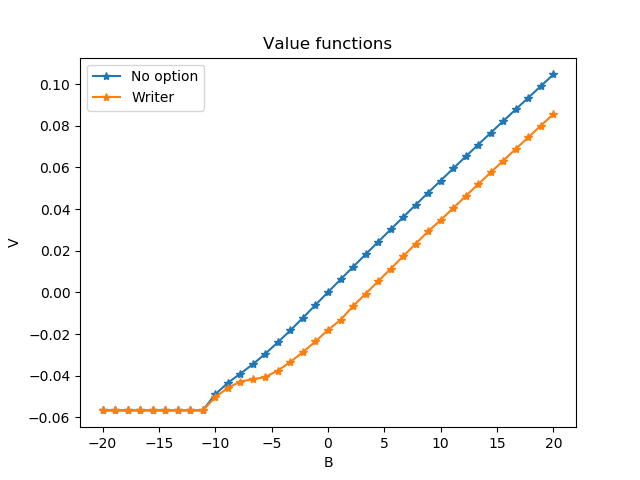
\includegraphics[width=\linewidth]{value_f_C10.png}
   \caption{Writer and no option value functions at $t_0$ with $C=10$, $Y_0=0$ and $S_0=15$.}
   \label{Fig23} 
 \end{minipage}
 \ \hspace{2mm} \hspace{3mm} \
 \begin{minipage}[b]{0.5\linewidth}
  %\centering
   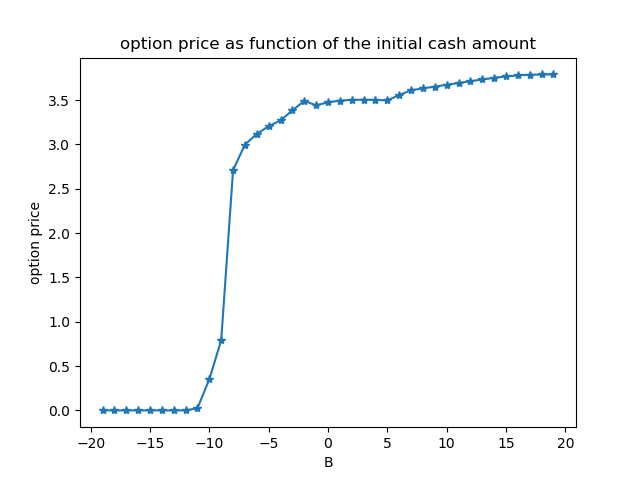
\includegraphics[width=\linewidth]{option_B.png}
   \caption{Option price as function of $B$ at $t_0$ with $C=10$, $Y_0=0$ and $S_0=15$.}
   \label{Fig24}
 \end{minipage}
\end{figure}  

It is important to stress that the grid resolution we used in these example is quite rough. The numerical results are still good, but it is not possible at the moment 
to study the convergence properties of the algorithm. 
Furthermore, although the value function is highly non-linear, we used linear interpolation to interpolate the missing points in the grid, and this may create further errors in the shape
of the function and in the final result.

\begin{figure}[t!]
 \begin{minipage}[b]{0.5\linewidth}
   \centering
   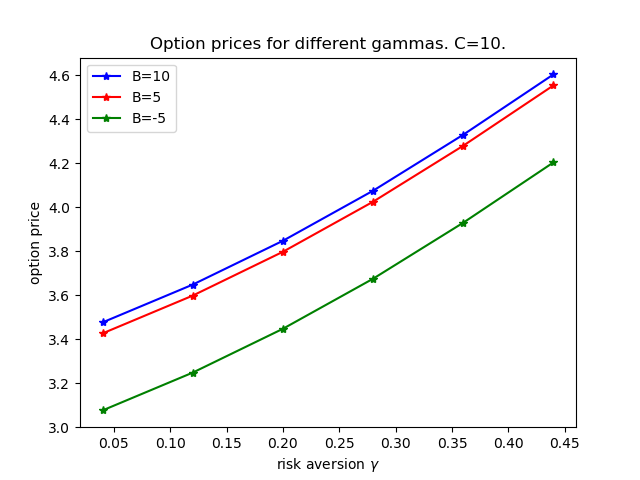
\includegraphics[width=\linewidth]{B_gamma_10.png}
   \caption{Option price as function of risk aversion, for several values of initial $B$. We set $C=10$, $Y_0=0$ and $S_0=15$.}
   \label{Fig26} 
 \end{minipage}
 \ \hspace{2mm} \hspace{3mm} \
 \begin{minipage}[b]{0.5\linewidth}
  %\centering
   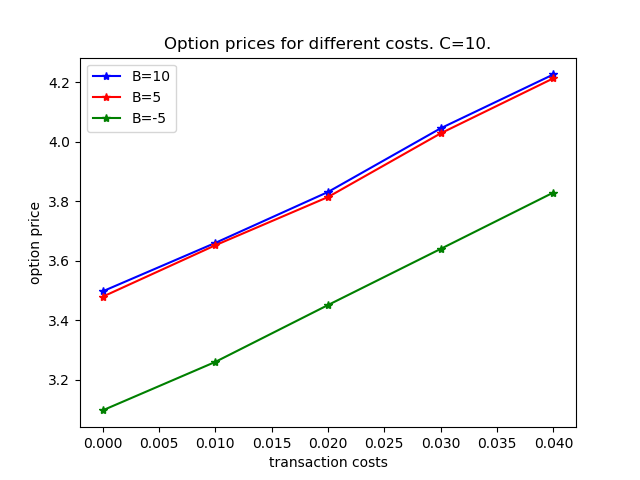
\includegraphics[width=\linewidth]{B_cost_10.png}
   \caption{Option price as function of transaction costs, for several values of initial $B$. We set $C=10$, $Y_0=0$ and $S_0=15$.}
   \label{Fig25}
 \end{minipage}
\end{figure}  

We conclude this section by testing the model properties as we did on Section \ref{model_properties}. 
In figures \ref{Fig26} and \ref{Fig25} we present several values of option prices as function of the risk aversion and transaction costs respectively.  
We can see that the value of $B$ does not affect the shape of the curve, but only its height. 
As we saw in figures \ref{Fig10} and \ref{Fig11}, the option price is an increasing function of the risk aversion and of the transaction costs.


\section{Multinomial method applied to the reduced problem}

In section \ref{MC_section} we have seen that a possible technique to construct the Markov chain approximation is to discretize the infinitesimal generator of the continuous process
by an explicit finite difference scheme.
For Lévy processes with infinite activity, however, this technique cannot be used directly,and requires to consider the infinitesimal generator of the approximated 
jump-diffusion process.
In the numerical results (section \ref{num_sec_VG}) we have also seen that the algorithm has a very slow time of convergence.\\
In this section we decide the use the multinomial approximation presented in Chapter \ref{Chapter3} instead of the discretization obtained by the infinitesimal generator.
We see that the gain in computational time is reduced. \\
Although the method still relies on an approximation (the VG process is approximated by a general jump process with only the first four moments equal),
with this method the number of branches is fixed to $\bar L = 5$, and therefore the computational complexity is reduced a lot.
Recall that the complexity for the general reduced variable algorithm is 
$$\mathcal{O}\biggl( (N+1)\bigl[\frac{N(\bar L-1)}{2}+1 \bigr] \times \bar M \times \bar M \biggr).$$
Assuming $\bar M = N$ and $\bar L = 5$, the computation time is reduced to $\mathcal{O}(N^4)$. 
\begin{table}[t!]
\begin{center}
\begin{minipage}{0.8\linewidth}
\centering
 \begin{tabular}{||c|c||}
 \hline
  \multicolumn{2}{|c|}{Convergence table} \\
  \hline
  $N = \bar M$ & Price \\
  \hline
    50 & 1.96121076540 \\
  \hline
    100 & 1.96889900730 \\
  \hline  
    200 &  1.97154200723 \\
  \hline
    400 & 1.97288296067 \\
  \hline   
    800 & 1.97354995910  \\
  \hline
    1000 & 1.97368292970 \\ 
  \hline
    1600 & 1.97388226442  \\
  \hline
    2000 & 1.97394872091  \\  \hline
  \end{tabular}
  \caption{Convergence table for ATM VG prices with parameters in Tab \ref{tab:VG}, calculated with the multinomial method.}
  \label{tab:convergence31}
\end{minipage}
 \end{center}
\end{table}
We use the values in table \ref{tab:VG} and follow the discretization scheme proposed in chapter \ref{Chapter3}. 
In table \ref{tab:convergence31} we reported a convergence analysis.
In the figures \ref{Fig32} and \ref{Fig33} we show how good are the prices computed with the multinomial method. 
\begin{figure}[t!]
 \begin{minipage}[b]{0.5\linewidth}
   \centering
   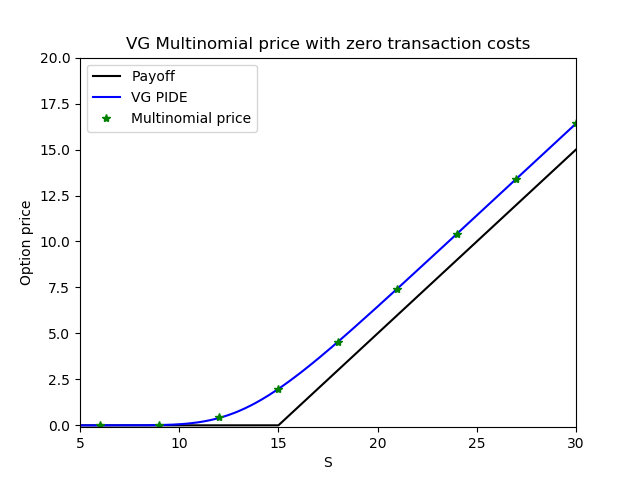
\includegraphics[width=\linewidth]{Multi_VG_zerocosts.png}
   \caption{The multinomial VG prices for zero transaction costs agree with the solution of the VG PIDE (continuous line).}
   \label{Fig32} 
 \end{minipage}
 \ \hspace{2mm} \hspace{3mm} \
 \begin{minipage}[b]{0.5\linewidth}
  %\centering
   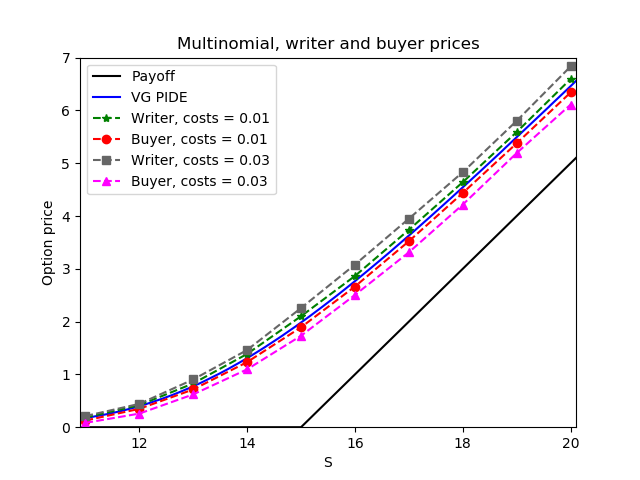
\includegraphics[width=\linewidth]{Multi_VG_costs.png}
   \caption{Multinomial VG writer and buyer prices for different transaction costs.}
   \label{Fig33}
 \end{minipage}
\end{figure}  

